
% PROjet d'enseignement

% Détails responsabilités filière

%   20% 

% Motivations pour l'enseignement

% 3 lettres reco
% copie des contrats

\documentclass[11pt]{article}
%\usepackage{makeidx}
%\usepackage{graphicx}
\usepackage[utf8]{inputenc}
\usepackage[OT1]{fontenc}
\usepackage[francais]{babel}
%\usepackage{a4wide}
\usepackage{fancybox}
%\usepackage{hyperref}
\usepackage{comment}
\usepackage{geometry}
\usepackage{eurosym}
\usepackage{amssymb}
\usepackage[pdftex]{graphicx}
\usepackage{pdfpages}

\usepackage{pgf}
\usepackage{pdfswitch}
\hypersetup{urlcolor=black,linkcolor=black,citecolor=black} % Keep printer friendly
%\geometry{hmargin=3.5cm, bottom=22mm,vmargin=2.5cm }
\geometry{top=23mm,bottom=27mm,left=17mm,right=27mm,headsep=0pt}
\setlength{\parindent}{1cm}


\usepackage[twoside,citeonce(page)]{footbib}
\usepackage{todonotes}

\footbibliography{generalbiblio}
\footbibliographystyle{plain}

\newcommand{\SG}[2][inline]{\todo[color=yellow!50,#1]{\sf \textbf{SG:} #2}}

\newcommand {\burl}[1]{\url{http://icps.u-strasbg.fr/~genaud/courses/#1}}

\newcommand {\rubrique}[1]{
\begin{flushleft}
{\large\bf #1}
\rule{\linewidth}{1mm}
\end{flushleft}
}
\newcommand{\pmpi}{\mbox{\textsc{P2P-MPI}}}


\makeatletter
\def\thebibliography#1{\subsection*{\rule{\linewidth}{1mm}\@mkboth
%\def\thebibliography#1{\subsection*{\rubrique{\large\bf Références biliographiques}\@mkboth
  {PUBLICATIONS}{PUBLICATIONS}}\list
      {[\arabic{enumi}]}{\settowidth\labelwidth{[#1]}\leftmargin\labelwidth
      \advance\leftmargin\labelsep
      \usecounter{enumi}}
      \def\newblock{\hskip .11em plus .33em minus .07em}
      \sloppy\clubpenalty4000\widowpenalty4000
      \sfcode`\.=1000\relax}
    \makeatother


\begin{document}
%------------------------- Page de Garde -------------------
%\setlength{\parskip}{0mm}
\thispagestyle{empty}
\vspace*{\stretch{1}}




\rule{\linewidth}{1mm}
\begin{center}
\Large{\textbf{Dossier de Candidature\\
aux fonctions de \\
Professeur des Universités\\
Poste 451 - UFR de Mathématiques-Informatique}}\\[5mm]
\Large{Stéphane \textsc{Genaud}}\\[1cm]

\rule{\linewidth}{1mm}
\vspace*{\stretch{2}}\\
\vspace{3cm}
%\DeclareGraphicsExtensions{.jpg}
%\includegraphics[width=5cm]{inria.jpg}
\end{center}
\begin{center}
Date: \today\\
\end{center}

\newpage
\mbox{}%blank page 

\setlength{\parindent}{5mm} %% restore a decnt value
\setlength{\parindent}{0mm}
%\setlength{\itemsep}{1mm}
\newpage


\begin{center}
\huge{\textsc{Table des matières}}
\end{center}
\vspace{2cm}


\tableofcontents

\noindent
%\rule{\linewidth}{0.3mm}


\newpage


%-------- C V -----------------------------------

\section{Curriculum Vit{\ae}}

\setlength{\tabcolsep}{5pt}

\subsection{\'Etat civil}

\medskip

\noindent
\begin{tabular}{llp{\linewidth}}

				%& \rule{\linewidth}{.2mm} \\
\hspace{1cm}	& Prénom et nom :			&\textbf{Stéphane GENAUD}\\
		 	& Date et lieu de naissance :	& Né le 10 mars 1969 à Forbach (57).\\
			& Nationalité :			& Française. \\
			& Situation familiale :		& Marié, 2 enfants. \\
			& Adresse professionnelle :	& LSIIT, Pôle API, Boulevard S. Brant,\\
			&      				& F-67400 Illkirch\\
			&					& Tél. : +33 (0)38 92 77 449\\ 
			&					& Fax  : +33 (0)3 90 24 45 47\\
			& Adresse électronique :	& \texttt{genaud@unistra.fr}\\
			& Page personnelle :		& \texttt{{\url{http://icps.u-strasbg.fr/members/genaud}}}\\[5mm]
				%& \rule{\linewidth}{.2mm} \\

\end{tabular}



\subsection{Formation Universitaire}
\medskip
\noindent
\begin{tabular}{lp{14.8cm}}
		%		& \rule{\linewidth}{.2mm} \\
	\textbf{2009} &  \textbf{Habilitation à diriger des recherches} en informatique \\
			  &	Université Henri Poincaré, Nancy. \textit{Soutenue le 8/12/2009}\\
      		  &	Titre du mémoire : {\em Exécutions de programmes parallèles à passage de messages sur grille de calcul}.\\
			  &	Jury~: 
				\begin{small}
				\begin{itemize}
				\item Pascal Bouvry (PU, Université du Luxembourg), Examinateur,
				\item Christophe Cérin (PU, Université Paris 13), Rapporteur,
				\item Frédéric Desprez (DR, INRIA Grenoble Rhônes-Alpes), Rapporteur,
				\item Claude Godart, (PU, Université Henri Poincaré), Président,
				\item Jens Gustedt (DR, INRIA Nancy Grand-Est), Garant,
				\item Thierry Priol (DR, INRIA Rennes Bretagne-Atlantique), Rapporteur.
				\end{itemize}
				\end{small}\\[2mm]
	

	\textbf{1997} & \textbf{Doctorat en Sciences, mention Informatique}\\
			  & Université Louis Pasteur, Strasbourg.\\
      		  & Titre du mémoire: {\em Transformations de programmes \textsc{Pei} : applications au parallélisme de données}.\\
		        & Jury~:
				\begin{small}
				\begin{itemize}
					\item Luc Bougé (PU, \'{E}NS Lyon), Rapporteur,
			    		\item Christian Lengauer (PU, Université Passau, Allemagne), Examinateur,
					\item Catherine Mongenet (PU, Université Louis Pasteur), Rapporteur interne,
					\item Guy-René Perrin (PU, Université Louis Pasteur), Directeur de thèse,
					\item Patrice Quinton (PU, Université de Rennes 1), Rapporteur.
				\end{itemize}
				\end{small}\\[2mm]
	\textbf{1993} &  \textbf{Diplôme d'\'{E}tudes Supérieures Spécialisées} (DESS) en Informatique du parallélisme, 
				  Université de Franche-Comté, Besançon. Mention {\em très bien} (major).\\[2mm]
	\textbf{1991} &  \textbf{Bachelor of Sciences} (BSc) in European Informatics, Sheffield Hallam University.\\[2mm]
%	\textbf{1989} &  {\bf Diplôme Universitaire de Technologie (DUT)} en informatique, Institut Universitaire de 
%					Technologies de Nantes, Université de Nantes.\\[5mm]
%		%	& \rule{\linewidth}{.2mm} \\

\end{tabular}
\newpage


\subsection{Expérience professionnelle}

\textit{Seules les expériences liées à une activité d'enseignement et/ou de recherche sont décrites ici.}\\[2mm]

\noindent
\begin{tabular}{p{2cm}p{14.3cm}}
%		& \rule{\linewidth}{.2mm} \\
% 	depuis sept. 2009 &  \textbf{Maître de conférences en Informatique} à l'Université de Strasbourg (UdS):\\[-7mm]
%		&\parbox[t]{13.7cm}{%
%            \begin{itemize}
%				  \item[$\rhd$] Enseignant à l'\'Ecole de Management Strasbourg,
%				  \item[$\rhd$] Chercheur au Laboratoire des Sciences de l'Image, de l'Informatique et de la Télédétection (LSIIT, UMR 7005 CNRS-UdS),
%équipe \textit{Image et Calcul Parallèle Scientifique} (ICPS).
%				\end{itemize}
%				\vspace{3mm}
% 				}\\

 	 \textbf{2007--2009}  &  \textbf{Détaché Chargé de Recherche} au Laboratoire Lorrain de Recherche en Informatique et ses Applications
(LORIA, UMR 7503 CNRS-INPL-INRIA-UHP-Nancy 2), équipe projet INRIA \textsc{AlGorille}.\\[2mm]

	\textbf{1998--2007}    &  \textbf{Maître de conférences en Informatique} à l'Université Robert Schuman, Strasbourg:\\[-3mm]
				&\parbox[t]{13.7cm}{%
                          \begin{itemize}
				  \item[$\rhd$] Enseignant à l'IECS, Université Robert Schuman,
				  \item[$\rhd$] Chercheur au LSIIT, UMR 7005 CNRS-ULP, équipe ICPS.
				\end{itemize}
				\vspace{3mm}
 				}\\


	\textbf{1996--1998} &  \textbf{Attaché Temporaire d'Enseignement et de Recherche} au département d'informatique 
de l'IUT de l'université Robert Schuman.\\[2mm]
	\textbf{1994--1996} & Doctorant à l'Université Louis Pasteur (ULP), Strasbourg. \\
				  & Directeur de thèse: Guy-René Perrin.\\[2mm]
	\textbf{1993--1994} & Doctorant à l'Université de Franche-Comté, Besançon. \\
				  & Directeur de thèse: Guy-René Perrin.\\[2mm]
%				& \rule{\linewidth}{.2mm} \\[5mm]

\end{tabular}

\vspace{6mm}
\textbf{\underline{Position administrative actuelle (depuis septembre 2009)}}
\vspace{5mm}

\begin{itemize}
\item
 	\textbf{Maître de conférences en Informatique} à l'Université de Strasbourg (UdS):
	\begin{itemize}
		\item Enseignant à l'\'Ecole de Management Strasbourg,
		\item Chercheur au Laboratoire des Sciences de l'Image, de 
		      l'Informatique et de la Télédétection \\
			(LSIIT, UMR 7005 CNRS-UdS).
équipe \textit{Image et Calcul Parallèle Scientifique} (ICPS).
\\[1mm]
	\end{itemize}

\item Titulaire de la \textbf{Prime d'Excellence Scientifique} depuis septembre 2009.\\

\item \textbf{Qualifié aux fonctions de Professeur des Universités} dans la 
              section 27 en 2010.\\
	\indent {\small Numéro de qualification~:~PR-2010-27-10127207589}\\[2mm]
\end{itemize}


\vspace{-1mm}
\subsection{Responsabilités principales}

\begin{itemize}
\item
 	\textbf{Responsabilités pédagogiques}
	\begin{itemize}
		\item Directeur délégué aux Systèmes d'Information de 
		      l'\'Ecole de Management Strasbourg depuis 07/2011.
		\item Responsable de la filière \textit{Système d'Information} 
		      du master Management International de l'IECS de 2002 à 2007.
	\end{itemize}
 	\textbf{Responsabilités recherche}
	\begin{itemize}
		\item Responsable du thème de recherche \textit{Grilles} dans 
		      l'équipe ICPS du LSIIT de 2001 à 2007. 
			Reprise du thème à mon retour dans l'équipe en septembre 2009.
		\item Membre du conseil scientifique du département \emph{Expertise 
		      pour la recherche de l'UdS} depuis 2010.
	\end{itemize}
 	\textbf{Responsabilités administratives et collectives}
	\begin{itemize}
		\item Membre de 3 commissions de spécialistes entre 2004 et 2008.
		\item Membre du comité d'experts UdS (section 27) depuis 2009 et 
		      membre dans 2 comités de sélection externes.
	      \item Co-responsable des systèmes d'information de mon 
		      établissement depuis 2001.
	\end{itemize}
\end{itemize}




%---------------------------- R E C H E R C H E --------------------------------
\newpage
\section{Activités de recherches}

\paragraph{Résumé}
\textit{Mes thèmes de recherche concernent le \emph{parallélisme}, 
essentiellement sur des architectures de type cluster, \emph{grilles} ou 
\emph{cloud}. Ma thèse de doctorat avait pour objet l'écriture et la 
transformation de programmes parallèles à l'aide d'un langage formel. A la 
suite de cette approche formelle, je me suis investi sur un problème réel dans 
le domaine de la  géophysique, nécessitant la conception et le développement 
d'applications parallèles. Lorsqu'ont émergé les grilles, j'ai étudié certains 
problèmes nouveaux que posaient ces systèmes hétérogènes, et la façon dont des 
applications pouvaient y être déployées. Mon travail sur les grilles a concerné 
l'évaluation et l'amélioration des performances des programmes parallèles dans 
ce contexte, puis l'amélioration des intergiciels pour mieux prendre en charge 
les programmes parallèles. L'utilisation des principes des systèmes pair-à-pair 
pour la découverte et l'auto-organisation des ressources ainsi que des 
mécanismes de tolérance aux pannes par réplication des calculs ont été proposés.
Parallèlement aux évaluations sur des cas et des plate-formes réelles, je 
travaille à la simulation de programmes distribués en contribuant à l'outil 
\textsc{SimGrid}. Je m'intéresse particulièrement à l'extension du simulateur 
pour permettre la simulation de programmes MPI sans modification du code source.
Enfin, mes recherches actuelles sont tournées vers les problèmes d'allocation 
des ressources et d'ordonnancement des tâches, dans le but de proposer aux 
clients de bons compromis performance/prix sur des plates-formes virtualisées 
comme celles fournies par les clouds IaaS.}\\ 

Ces différents aspects sont détaillés ci-après, puis suivent la liste de mes 
publications, mon activité d'animation scientifique, mes participations à des 
encadrements, et mes perspectives de recherches.

\subsection{Détails des thèmes de recherche}


\subsubsection{\textsc{Pei}}

Ma thèse de doctorat \cite{icps-1997-4} a porté sur la définition et 
l'utilisation d'un langage formel baptis\'e Pei~\footcite{Violard92}. Ce 
formalisme permet la description de programmes pour des ordinateurs parallèles, 
dans un modèle de programmation de type \emph{parallélisme de données}. Nous 
avons montré comment ce formalisme pouvait être utilisé pour raisonner sur les 
programmes et les transformer en nouveaux programmes sémantiquement 
équivalents ou raffinés \cite{icps-1994-46,icps-1995-1,icps-1997-3,icps-1996-2}.
Le deuxième volet du travail a consisté à proposer des méthodes pour traduire
ces énoncés formels vers des langages parallèles cibles comme 
\textit{High Performance Fortran} ainsi que les logiciels permettant les 
transformations, le contrôle de validité des programmes ainsi que les 
compilateurs pour la traduction%
\footnote{\url{http://icps.u-strasbg.fr/pei/PEI_SUMMARY/langage.htm}}.


\subsubsection{Parallélisation pour la géophysique}

%..............................................................................|80
Après cette expérience d'approche formelle d'un modèle de programmation pour 
le parallélisme, je me suis plongé dans un travail concret de parallélisation 
sur des codes scientifiques. Je me suis investi en particulier dans la 
conception et le développement d'outils logiciels pour la géophysique. L'enjeu 
est de pouvoir calculer une tomographie sismique globale en ondes de volumes 
permettant d'améliorer un modèle de vitesses des ondes sismiques, et de là 
en déduire des propriétés géologiques à l'intérieur de la Terre. L'ensemble 
de ces outils\footnote{\url{http://renass.u-strasbg.fr/ray2mesh}} conçus lors 
d'une thèse en collaboration avec l'Institut de Physique du Globe de Strasbourg 
(UMR CNRS-UdS 7516) permet de combiner et d'enchaîner des traitements sur des 
données géophysiques extrêmement volumineuses. Le travail s'est concrétisé par 
une tomographie utilisant la totalité des données (sismogrammes) acquises 
depuis 1965 par les réseaux de surveillances sismiques à travers le monde. Pour 
répondre à cet objectif les applications ont été conçues pour s'exécuter sur 
des architectures parallèles, et ont été testées sur des configurations très 
différentes allant de la machine parallèle à des réseaux de station de travail 
en passant par des grilles de calcul (cf. paragraphe suivant) à l'échelle 
nationale~\cite{icps-2005-146,icps-2007-184}.  


\subsubsection{Grilles de calcul}

%..............................................................................|80
L'exploitation de telles applications scientifiques pose des problèmes concrets 
quant au choix de la machine cible pour l'exécution. Un type d'architecture 
nouveau a émergé ces dernières années grâce aux technologies qui permettent
de fédérer efficacement des ressources de calcul provenant d'institutions 
différentes. Cette alternative a été popularisée~\footcite{Foster97,Foster98} 
sous l'appellation de \emph{grilles}. J'ai porté en 2001 un projet intitulé 
\textit{Transformations et Adaptations de programmes pour la Grille} (TAG)
accepté dans le cadre de l'Action Concertée Incitative (ACI) Grid du Ministère 
de la Recherche (2002--2005). Le projet visait l'étude du comportement 
d'applications scientifiques, essentiellement des programmes MPI~\footnote{%
Message Passing Interface définit une bibliothèque de fonctions permettant 
à des processus d'échanger des messages. C'est devenu le standard \textit{de 
facto} pour les programmes parallèles exécutés sur des architectures à mémoire 
distribuée.} sur les grilles. Deux catégories de problèmes ont été traitées 
dans ce projet. D'une part, déterminer quelles \emph{performances} on peut 
espérer d'une application exécutée sur des ressources hétérogènes distribuées 
à large échelle géographique et ce qu'on peut faire pour les améliorer.
D'autre part, travailler sur la couche \emph{intergicielle} pour masquer la 
complexité de ces systèmes répartis et améliorer la prise en charge des 
applications.


\paragraph{Performances} 

Pour améliorer les performances, une partie de mon travail a été l'étude de 
techniques d'équilibrage de charge statiques ou dynamiques.  En effet, les 
découpages des données et la distribution de la charge dans de nombreuses 
applications parallèles font l'hypothèse que les processeurs et les réseaux 
sont homogènes. Pour optimiser le temps de calcul d'un ensemble de tâches
indépendantes exécutées sur des processeurs hétérogène, il faut déterminer la 
meilleure quantité de données distribuées à chacune. Nous avons proposé des 
algorithmes pour déterminer statiquement de telles distributions optimales. Ces
algorithmes ont été testés sur de vraies applications, dont l'application de 
géophysique décrite précédemment~\cite{icps-2002-62,icps-2003-75,icps-2004-125}. 
Nous avons également comparé cette approche statique à l'approche dynamique 
dans laquelle le maître distribue un nouveau bloc de travail à un esclave dès 
que celui-ci le demande : l'équilibrage de charge se fait alors naturellement 
selon le rythme de calcul des esclaves. La difficulté dans cette approche est 
de déterminer la taille du bloc à envoyer: en dessous de la taille idéale, il y 
a des aller-retours inutiles, tandis qu'au dessus, les esclaves ne finissent 
pas simultanément. En revanche, cette stratégie possède l'avantage majeur
de s'adapter aux variations de charge.


\paragraph{Intergiciel}

Les travaux précédents se sont largement appuyés sur l'expérimentation réelle
sur des grilles construites avec le logiciel Globus. La prise en charge de nos 
applications par cet intergicel ne correspondant pas à nos attentes, nous avons 
proposé un nouveau type d'intergiciel spécialisé pour MPI. Parmi les 
lacunes observées pour l'exécution des programmes parallèles figurent l'absence 
de mécanisme de co-allocation de ressources sur différents sites, la détection 
de la disponibilité des ressources au moment précis de l'exécution, la gestion 
de binaires multiples pour chaque systèmes, la difficulté d'accéder aux fichiers
de données et programmes, et l'absence de détection des pannes et de tolérance 
aux pannes. Nous avons développé {\pmpi}\footnote{~\url{http://www.p2pmpi.org}},
pour pallier ces lacunes. {\pmpi} comprend à la fois la couche intergicielle et 
la bibliothèque de communication permettant de développer des programmes 
parallèles à passage de messages. Cette dernière est une implémentation de 
MPJ\footnote{Message Passing for Java: adaptation de MPI pour Java}qui intègre 
la notion de tolérance aux pannes. Les applications sont des programmes Java, 
beaucoup plus faciles à déployer dans un environnement hétérogène.
Pour la couche intergicielle, nous reprenons les principes des systèmes 
pair-à-pair: chaque machine démarrée avec {\pmpi} devient un pair susceptible 
de partager son CPU ou d'utiliser ceux des autres. Cette approche confère 
autonomie et robustesse aux applications. L'autonomie provient de la 
possibilité de découvrir dynamiquement un ensemble de pairs disponibles à ce 
moment précis pour exécuter un programme parallèle. On construit ainsi 
dynamiquement une ``plate-forme'' à chaque demande d'exécution. La façon de 
choisir les pairs les plus adaptés parmi ceux disponibles dépend de plusieurs 
critères, dont la latence réseau qui sépare la machine qui fait la requête des 
pairs candidats, la présence ou non des données nécessaires dans les caches des 
pairs distants, et le souhait de l'utilisateur de concentrer ou non les 
processus sur le minimum de machines. 

Dans de tels systèmes, les pannes sont fréquentes. Or, lors d'un calcul, la 
panne d'un des participants provoque l'arrêt de l'application. Pour diminuer le 
risque de panne, nous avons proposé une solution jamais expérimentée dans ce 
contexte qui est la réplication des calculs. L'utilisateur décide du taux de 
redondance de l'exécution de chaque processus, sur des machines différentes, et 
le système gère de manière transparente la cohérence de l'exécution. En cas de 
panne de l'un des processus, l'application peut poursuivre son exécution tant 
qu'il subsiste au moins une copie de ce processus de calcul.\\


La conception de {\pmpi} à été décrite dans~\cite{icps-2007-182,icps-2005-155}.
Nous avons aussi démontré sa capacité à prendre en charge l'exécution de 
programmes parallèles sur plusieurs centaines de processeurs~%
\cite{icps-2008-193}. La thèse de Choopan Rattanapoka~\footcite{icps-2008-208} 
présente l'ensemble des résultats. {\pmpi} est aussi un support pour l'étude de 
la tolérance aux pannes. Nous avons étudié le mécanisme de réplication des 
calculs que nous proposons~\cite{icps-2007-185} en montrant comment déterminer 
un taux optimal de réplication~\cite{icps-2009-217} puis en faisant une étude 
quantitative du coût de la réplication et des temps de reprise~%
\cite{icps-2009-214}.

Enfin, je me suis attaché à valider notre proposition sur de vraies 
applications.Deux collaborations ont abouties dans ce cadre. En 2007 et 2008 
nous avons aidé des collègues du LSIIT (Pierre Gançarski), dans le domaine de 
la fouille de données, à paralléliser leur méthode d'apprentissage non-%
supervisée pour le clustering~\cite{icps-2008-188}. En 2008 et 2009, nous avons 
collaboré avec des collègues de SUPELEC (Virginie Galtier et Stéphane Vialle) 
pour comparer les implantations parallèles de la méthode d'apprentissage 
Adaboost dans deux modèles de programmation différents (JavaSpace et MPJ)~%
\cite{icps-2009-219}.


\subsubsection{Simulation}
\label{sc:simulation}

Les expérimentations que nous avons menées dans notre travail sur les grilles 
ont été fastidieuses. L'apparition de l'outil Grid'5000 a considérablement
élargi les possibilités d'expérimentation dans un environnement réel, tout
en permettant un protocole expérimental plus rigoureux car l'utilisateur
peut sélectionner le matériel voulu, et installer le système d'exploitation de
son choix. Le caractère reproductible des expériences a donc été considérablement
amélioré avec Grid'5000, mais reste néanmoins imparfait, car le
réseau reliant les sites ainsi que les clusters sont régulièrement renouvelés.
Les expériences doivent donc se succéder sur une période relativement courte
pour obtenir une série de résultats comparables. Cependant, les problèmes 
techniques ou la difficulté d'obtenir l'accès à l'outil au moment souhaité 
peuvent fortement allonger la période d'expérimentation.
La simulation présente face à ce problème un grand intérêt. Elle peut permettre
de tester de nombreux scénarios, et de ne faire des expériences réelles que pour
les cas les plus intéressants.\\

\textsc{SimGrid}~\footcite{Casanova08} est un projet important dans le paysage 
de la recherche académique sur la simulation des systèmes distribués. Le 
logiciel permet de décrire l'ensemble des ordinateurs connectés et le réseau 
les interconnectant, ainsi que les opérations de calcul et de communication 
survenant au sein d'une application, et d'en faire une simulation à évènements 
discrets. Le déroulement d'une application est décrit à travers une 
\emph{interface} au simulateur, c'est-à-dire une API fournie pour décrire ces 
opérations de calcul et de communication.\\

Ce logiciel a été soutenu entre autres par le projets ANR USS-SimGrid%
\footnote{\url{http://uss-simgrid.gforge.inria.fr/}} 
\footnote{Labelisé projet \textit{phare} par l'ANR.}
(2009-2011), puis aujourd'hui par le projet SONGS%
\footnote{\url{http://infra-songs.gforge.inria.fr/}} 
(2012-2015). Je participe à ces projets, dont l'objectif est d'étendre les 
capacité de l'outil. Il n'existait pas par exemple, avant le projet Uss-Simgrid,  
d'interface permettant de simuler les programmes parallèles à passage de 
messages (ses deux principales API proposaient alors des communications point à 
point bloquantes). Nous avons proposé une interface pour simuler des programmes 
MPI. J'ai réactivé un effort fait dans ce sens à l'université d'Hawaï (Mark 
Stillwell et Henri Casanova) mais inachevé, baptisée SMPI. Ce travail, poursuivi 
par Pierre-Nicolas Clauss a abouti à une version désormais livrée avec SimGrid. 
La conception et l'évaluation de SMPI ont fait l'objet d'une publication à la 
conférence IPDPS~\cite{icps-2011-224}. Plusieurs perspectives sont ouvertes avec 
cet outil. On peut extrapoler l'exécution d'un programme sur une machine qui 
n'existe pas encore, dont on ne donne que la description. Ceci peut servir par 
exemple à des fins de dimensionnement d'un cluster. Cela peut être utile dans 
de nombreuses autres situations, comme l'enseignement, où une machine de bureau 
peut servir à simuler un clusterou un système distribué. On peut également 
imaginer dans le futur continuer des exécutions en simulation après avoir 
capturé la trace d'un programme réellement exécuté (avec des outils de 
profiling existants) et en injectant cette trace dans le simulateur.




%----------------- P U B L I C A T I O N S ---------------------------
\newpage

\subsection{Liste de publications}


\small
\bibliographystyle{plain}
\begin{thebibliography}{99}

\subsection*{Thèses}

\bibitem{hdr}
\textbf{Stéphane Genaud}.
\newblock {\em Exécutions de programmes parallèles à passage de messages sur grille de calcul}.
\newblock Habilitation à diriger des recherches de l'université Henri Poincaré, Nancy. Décembre 2009.
\newblock Rapporteurs : C. Cérin (Paris 13), F. Desprez (INRIA Rhônes-Alpes), T. Priol (INRIA Bretagne-Atlantique).\\[2mm]

\bibitem{icps-1997-4}
\textbf{Stéphane Genaud}.
\newblock {\em Transformations de programmes \textsc{Pei} : applications au
  parallélisme de données}.
\newblock Thèse de doctorat de l'université Louis Pasteur, Strasbourg, Janvier 1997.
\newblock Rapporteurs : Luc Bougé et Patrice Quinton. 

\subsection*{Chapitre de livre}

\bibitem{icps-book}
\textbf{Stéphane Genaud} et Choopan Rattanapoka.
\newblock \emph{A Peer-to-Peer Framework for Message Passing Parallel Programs.}
\newblock Parallel Programming and Applications in Grid, P2P and Network-based System,
in {\em Advances In Parallel Computing} Series. Editor Prof. Dr. Gerhard R. Joubert.
IOS Press, juin 2009. 
 

\subsection*{Articles en revues internationales}

\setlength{\itemsep}{1.5mm}


\bibitem{icps-2009-217}
\newblock \textbf{Stéphane Genaud}, Emmanuel Jeannot et Choopan Rattanapoka.
\newblock Fault-Management in P2P-MPI.
\newblock {\em International Journal of Parallel Programming}, Springer, 
37(5):433--461, août 2009.


\bibitem{icps-2008-188}
\textbf{Stéphane Genaud}, Pierre Gançarski, Guillaume Latu, Alexandre Blansché, 
Choopan Rattanapoka et Damien Vouriot. \newblock Exploitation of a parallel 
clustering algorithm on commodity hardware with P2P-MPI.
\newblock {\em The Journal of SuperComputing}, Springer, 43(1):21--41, jan. 2008.


\bibitem{icps-2007-182}
\textbf{Stéphane Genaud} et Choopan Rattanapoka.
\newblock P2P-MPI: A Peer-to-Peer Framework for Robust Execution of Message Passing Parallel Programs on Grids.
\newblock {\em Journal of Grid Computing}, Springer, 5(1):27--42, mai 2007.


\bibitem{icps-2004-125}
\textbf{Stéphane Genaud}, Arnaud Giersch, et Frédéric Vivien.
\newblock Load-balancing scatter operations for Grid computing.
\newblock {\em Parallel Computing}, Elsevier, 30(8):923--946, août 2004.

\bibitem{icps-2004-107}
Marc Grunberg, \textbf{Stéphane Genaud} et Catherine Mongenet.
\newblock Seismic ray-tracing and Earth mesh modeling on various parallel
  architectures.
\newblock {\em The Journal of Supercomputing}, Kluwer, 29(1):27--44, juillet 2004.


\subsection*{Articles en revues nationales}
\bibitem{icps-2005-146}
\textbf{Stéphane Genaud} et Marc Grunberg. 
\newblock  Calcul de rais en tomographie sismique : exploitation sur la grille.
\newblock {\em Technique et Science Informatiques}, numéro spécial Renpar, 
Hermès-Lavoisier, 24(5), pages 591--608, décembre 2005.

\bibitem{icps-1996-2}
\textbf{Stéphane Genaud}.
\newblock Transformations d'énoncés \textsc{Pei}.
\newblock {\em Technique et Science Informatiques}, 15(5), pages 601--618, 
Hermès, avril 1996.

\bibitem{icps-1993-69}
\textbf{Stéphane Genaud} et Guy-René Perrin.
\newblock Une expérience d'implantation d'un algorithme systolique sur
  hypercube.
\newblock {\em La Lettre du Transputer et des calculateurs parallèles},
  (17), mars 1993.


\subsection*{Conférences internationales avec actes et comité de lecture}

\bibitem{icps-2011-225}
\newblock \textbf{Stéphane Genaud} et Julien Gossa,
\newblock Cost-wait Trade-offs in Client-side Resource Provisioning with 
Elastic Clouds.
\newblock {\em 4th IEEE International Conference on Cloud Computing (CLOUD 
2011)}, juillet 2011.
\newblock \small{\textit{(papiers acceptés/soumis{:}36/198, taux: 18\%)}}


\bibitem{icps-2011-224}
\newblock Pierre-Nicolas Clauss, Mark Stillwell, \textbf{Stéphane Genaud}, 
Fr\'ed\'eric Suter, Henri Casanova and  Martin Quinson.
\newblock Single Node On-Line Simulation of MPI Applications with SMPI.
\newblock {\em 25th IEEE International Parallel \& Distributed Processing 
Symposium (IPDPS 2011)}, mai 2011.
\newblock \small{\textit{(papiers acceptés/soumis{:}112/571, taux: 19\%)}}

\bibitem{icps-2009-219}
\newblock Virginie Galtier, \textbf{Stéphane Genaud} et Stéphane Vialle.
\newblock Implementation of the AdaBoost Algorithm for Large Scale Distributed 
Environments: Comparing JavaSpace and MPJ.
\newblock {\em International Conference on Parallel and Distributed Systems}, 
IEEE, déc. 2009.
\newblock \small{\textit{(papiers acceptés/soumis:91/305, taux: 29\%)}}


\bibitem{icps-2009-214}
\textbf{Stéphane Genaud} and Choopan Rattanapoka.
\newblock Evaluation of Replication and Fault Detection in P2P-MPI.
\newblock {\em 6th IEEE International Workshop on Grid Computing (HPGC), IPDPS 2009}, mai 2009.
\newblock \textit{(Papier invité)}.

\bibitem{icps-2008-193}
\textbf{Stéphane Genaud} and Choopan Rattanapoka. 
\newblock Large-Scale Experiment of Co-allocation Strategies for Peer-to-Peer Supercomputing in P2P-MPI,
\newblock {\em 5th IEEE International Workshop on Grid Computing (HPGC), IPDPS 2008}, avril 2008.

\bibitem{icps-2007-192}
Ludovic Hablot and Olivier Glück and Jean-Christophe Mignot and \textbf{Stéphane Genaud} and Pascale Vicat-Blanc Primet.
\newblock Comparison and tuning of MPI implementation in a grid context.
\newblock {\em Proceedings of 2007 IEEE International Conference on Cluster Computing (CLUSTER)}, 458--463, september 2007.
\newblock \small{\textit{(papiers acceptés/soumis:42/106, taux: 39\%)}}

\bibitem{icps-2007-185}
\newblock \textbf{Stéphane Genaud} et Choopan Rattanapoka.
\newblock Fault Management in {\pmpi}. 
\newblock International Conference on {\em Grid and Pervasive Computing, (GPC 2007)}, LNCS, Springer, mai 2007.
\newblock \small{\textit{(papiers acceptés/soumis:56/217, taux: 25\%)}}
%submitted papers: 217; accepted : 56 full papers, 12 oral-short papers;  acceptance rate: 25\%

\bibitem{icps-2007-184}
\newblock \textbf{Stéphane Genaud}, Marc Grunberg et Catherine Mongenet.
\newblock Experiments in running a scientific {MPI} Application on GRID'5000. 
\newblock distingué par le \textsc{Intel} \textit{best paper award}.
\newblock {\em 4th IEEE International Workshop on Grid Computing (HPGC), IPDPS 2007}, mars 2007.


\bibitem{icps-2005-155}
\textbf{Stéphane Genaud} et Choopan Rattanapoka.
\newblock A Peer-to-peer Framework for Robust Execution of Message Passing Parallel Programs.
\newblock In {\em EuroPVM/MPI 2005}, LNCS 3666, Springer-Verlag, pages 276--284, septembre 2005.
\newblock \small{\textit{(papiers acceptés/soumis:61/126, taux: 48\%)}}


\bibitem{icps-2004-124}
Marc Grunberg, \textbf{Stéphane Genaud}, et Catherine Mongenet.
\newblock Parallel adaptive mesh coarsening for seismic tomography.
\newblock In {\em SBAC-PAD 2004, 16th Symposium on Computer Architecture and
  High Performance Computing}. IEEE Computer Society Press, octobre 2004.
\newblock \small{\textit{(papiers acceptés/soumis:32/93, taux: 34\%)}}

\bibitem{icps-2003-75}
\textbf{Stéphane Genaud}, Arnaud Giersch, et Frédéric Vivien.
\newblock Load-balancing scatter operations for Grid computing.
\newblock In {\em Proceedings of 12th Heterogeneous Computing Workshop 
(HCW), IPDPS 2003}. IEEE Computer Society Press, avril 2003.

\bibitem{icps-2002-62}
Romaric David, \textbf{Stéphane Genaud}, Arnaud Giersch, \'{E}ric Violard, et 
  Benjamin Schwarz.
\newblock Source-code transformations strategies to load-balance Grid
  applications.
\newblock In {\em International Conference on Grid Computing - GRID'2002}, LNCS 2536,
  pages 82--87. Springer-Verlag, novembre 2002.

\bibitem{icps-2002-20}
Marc Grunberg, \textbf{Stéphane Genaud}, et Catherine Mongenet.
\newblock Parallel seismic ray-tracing in a global {E}arth mesh.
\newblock In {\em Proceedings of the 2002 Parallel and Distributed Processing
  Techniques and Applications (PDPTA'02)}, pages 1151--1157, juin 2002.

\bibitem{icps-1997-3}
Eric Violard, \textbf{Stéphane Genaud} et Guy-René Perrin.
\newblock Refinement of data-parallel programs in pei.
\newblock In {\em IFIP Working Conference on Algorithmic Language and Calculi}, 
R.~Bird and L.~Meertens editors, Chapman \& Hall~Ed., février 1997.
\newblock 25 pages.

\bibitem{icps-1995-1}
\textbf{Stéphane Genaud}, Eric Violard, et Guy-René Perrin.
\newblock Transformation techniques in \textsc{Pei}.
\newblock In P.~Magnusson S.~Haridi, K.~Ali, editor, {\em Europar'95}, LNCS
  966, pages 131--142. Springer-Verlag, août 1995.
\newblock \small{\textit{(papiers acceptés/soumis:50/180, taux: 27\%)}}




\subsection*{Conférences nationales avec actes et comité de lecture}
\bibitem{icps-2003-111}
Marc Grunberg et \textbf{Stéphane Genaud}.
\newblock Calcul de rais en tomographie sismique : exploitation sur la grille.
\newblock In {\em Renpar2003}, pages 179--186. INRIA, octobre 2003.

\bibitem{icps-1995-6}
\textbf{Stéphane Genaud}.
\newblock Techniques de tranformations d'énoncés \textsc{Pei} pour la
  production de programmes data-parallèles.
\newblock In {\em RenPar 7}, mai 1995, Mons, Belgique.

\bibitem{icps-1994-46}
Guy-René Perrin, Eric Violard et \textbf{Stéphane Genaud}.
\newblock \textsc{Pei} : a theoretical framework for data-parallel programming.
\newblock In {\em Workshop on Data-Parallel Languages and Compilers}, Lille, mai 1994.
\vspace{3mm}


\subsection*{Autres communications}

\bibitem{iphc-2011}
Christine Carapito, Jérôme Pansanel, Patrick Guterl, Alexandre Burel, Fabrice 
Bertile, \textbf{Stéphane Genaud}, Alain Van Dorsselaer, Christelle Roy.
\newblock Une suite logicielle pour la protéomique interfacée sur une grille de 
calcul. Utilisation d'algorithmes libres pour l'identification MS/MS, le 
séquençage de novo et l'annotation fonctionnelle.
\newblock Rencontres Scientifiques France Grilles 2011, Lyon.

\bibitem{cds-2005}
A. Schaaff, F. Bonnarel, J.-J. Claudon, R. David, \textbf{S. Genaud}, M. Louys, C. Pestel and C. Wolf, 
\newblock Work around distributed image processing and workflow management, 
\newblock poster à ADASS 2005, Madrid.


\bibitem{icps-2003-113}
Marc Grunberg, \textbf{Stéphane Genaud}, et Michel Granet.
\newblock Geographical {ISC} data characterization with parallel ray-tracing.
\newblock In {\em Eos Trans. AGU, 84(46), Fall-Meeting Suppl., Abstract
  S31E-0793}, décembre 2003.

\bibitem{icps-2003-114}
\textbf{Stéphane Genaud}.
\newblock Applications parallèles sur la grille: mieux vaut il être rapide ou résistant ? 
\newblock {\em Actes de GridUSe-2004}, Workshop "What we have learned", conférence invitée.
\newblock Supélec Metz, juin 2004. 

\subsection*{En cours de soumission}

\bibitem{itpro-cs11}
\newblock \textbf{Stéphane Genaud}, Julien Gossa et Etienne Michon.
\newblock Provisioning Cloud resources on the client-side: a cost-performance trade-off approach.
IEEE IT Professional Magazine on Cloud Computing. Nov 2011

\bibitem{tomacs-11}
Olivier Beaumont, Laurent Bobelin, Henir Casanova, Pierre-Nicolas Clauss, 
Bruno Donassolo, Lionel Eyraud-Dubois, \textbf{Stéphane Genaud}, Sacha Hunold, 
Arnaud Legrand, Martin Quinson.
\newblock
Towards Scalable, Accurate, and Usable Simulations of Distributed Applications and Systems,
ACM Transactions on Modeling and Computer Simulation. Oct 2011.

\bibitem{michon2012}
Etienne Michon, Julien Gossa, \textbf{Stéphane Genaud}.
\newblock Free elasticity and free CPU power on IaaS Clouds: Promises and Study.
Europar 2012. Fev 2012.
\end{thebibliography}


%-----------------A N I M A T I O N -------------------
\subsection{Activités scientifiques}

\subsubsection{Niveau international}
Membre des comité de programmes des conférences internationales:\\[-3mm]
\begin{itemize}
\item[$\bullet$] 
14th IEEE International Conference on High Performance Computing and Communications (HPCC 2012), 
2012 (Liverpool, England),
\item[$\bullet$] 
13th IEEE International Conference on High Performance Computing and Communications (HPCC 2011), 
2011 (Banff, Canada),
\item[$\bullet$] 
IEEE/ACM International Conference on Grid Computing (GRID'10), 2010 (Bruxelles, Belgique),
\item[$\bullet$] 
20th IASTED International Conference on Parallel and Distributed Computing and Systems, 2010, (Marina Del Rey, USA),
\item[$\bullet$] 
IEEE/ACM International Conference on Grid Computing (GRID'08), 2008 (Tsukuba, Japon), 
\item [$\bullet$]
International Symposium on Grid and Distributed Computing, 2008 (Hainan Island, Chine),\\
\end{itemize}

Relecteur pour de nombreuses revues ou conférences internationales: IEEE Trans. on Distr. and Parallel Systems, 
J. of SuperComputing, J. of Grid Computing, IEEE Conference on Grid Computing, IEEE CCGrid conference, Europar,
IEEE IPDPS conference, \ldots.


\subsubsection{Niveau national}
%------------------------------------
\begin{itemize}

\item[$\bullet$] Obtention de la prime d'excellence scientifique (PES) à partir d'octobre 2009.\\

\item [$\bullet$]
membre du comité de rédaction de la revue Technique et Science Informatiques (2005--2009).\\
\end{itemize}

\underline{Projets en cours}\\
\begin{itemize}


\item[$\bullet$]
\textbf{Porteur local} pour le projet ANR SONGS (ANR 11 INFR 013-03)  (taux déclaré 40\%)
coordonné par Martin Quinson, LORIA, Nancy (2012-2015)  poursuivant le projet 
Uss-SimGrid (voir ci-dessous). Le projet vise à affiner les objets modélisés pour la 
simulation (processeurs multi-c{\oe}eurs, mémoire) ou en ajouter (disque, réseaux spécialisés
comme Infiniband) et à fournir des interfaces adaptées à la représentation de systèmes
complexes comme des machines HPC ou des Clouds. Je suis responsable du work package
sur les clouds.\\

\item[$\bullet$]
Participant au projet blanc ANR E2T2 (ANR 11 SIMI 9) (taux déclaré 15\%) coordonné par 
Peter Beyer, laboratoire PIIM, Université de Provence (2011-2014). L'objectif du projet 
est d'améliorer la modélisation physique des plasmas de bord dans un tokamak. Dans ce
projet, ma tâche est de co-encadrer un doctorant, Matthieu Kuhn avec Guillaume Latu et
Nicolas Crouseille (IRMA) pour paralléliser les codes développés par le CEA Cadarache 
(IRFM) et les physiciens du PIIM. \\

\item[$\bullet$]
\textbf{Co-animateur} d'une action d'animation scientifique 
dans le cadre de l'action de développement technologique (ADT) de Aladdin de l'INRIA, 
visant à pérenniser l'outil scientifique Grid5000. (07/2008--06/2012). 
Conjointement à l'ADT, l'animation scientifique est organisée autour de neuf actions d'animations baptisées \emph{défis}.
Je co-anime avec Nouredine Melab (LIFL, Université de Lille) le défi 
``{\em scalable application for large scale systems (algorithm, programming, execution models)}''.\\
\end{itemize}


\underline{Projets passés}\\
\begin{itemize}
\item[$\bullet$]
Participant (taux déclaré 20\%) au projet ANR USS-SimGrid (ANR 08 SEGI 022) coordonné par 
Martin Quinson, LORIA, Nancy (2009 -- 2011). Ce projet a été labelisé projet \textit{phare}
par l'ANR.
L'objectif général du projet était  d'élargir les capacités 
de l'environnement de simulation SimGrid pour satisfaire des besoins plus divers, comme la
simulation de systèmes pair-à-pair ou d'environnements de calcul intensif.
Mes tâches ont concerné l'enregistrement des traces d'exécutions (des programmes MPI en 
particulier) afin de les rejouer dans le simulateur. J'ai redémarré
le travail commencé à l'université de Hawaï sur l'interface SMPI, qui permet de simuler des 
programmes MPI sans modification des codes sources. Elle est maintenant fonctionnelle depuis
la version 3.5 de SimGrid.\\


\item[$\bullet$]
Participant (taux déclaré 20\%) au projet SPADES (ANR 08 SEGI 025) coordonné par Eddy Caron, 
LIP-ENS Lyon (2009 -- 2011). L'objectif était de concevoir et construire un intergiciel capable 
de gérer un environnement dans lequel la disponibilité des ressources change très rapidement. 
En particulier, cet intergiciel doit donner accès de manière fugace à des équipements de calculs 
très haute performance. Mes tâches ont concerné la conception et l'évaluation de l'ordonnanceur
travaillant en collaboration avec un système pair-à-pair utilisé pour recenser dynamiquement
les ressources disponibles.\\


\item[$\bullet$] Participant (10\%) au projet Masse de Données Astronomiques (ACI Masse de données) 
coordonné par Françoise Genova, observatoire de Strasbourg (2004 -- 2006). \\

\item[$\bullet$]
\textbf{Porteur d'un projet d'Action Concertée Incitative}. Projet TAG, 
pluridisciplinaire dans de l'ACI GRID (Globalisation des ressources informatiques et des données) 
du ministère de la recherche. Doté d'un budget de 182 K\euro{} et d'un poste d'ingénieur). 
(12/2001 -- 12/2003).\\
\end{itemize}


%\item Orateur dans diverses manifestations scientifiques sur ma thématique de recherche 
% * Journées \textit{Grilles} du CINES en mars 2003 à Montepllier, 
% * conférence et papier invité à GridUSe-2004 au workshop "What we have learned" 
%   de l'école thématique sur la \textit{globalisation des ressources informatiques et des données : Utilisation et Services},
%   juin 2004, Supélec Metz). 
% * Exposé Invité, Paristic 2006, 23 nov 2006, LORIA. Track 'Grid5000'. 
%   "Extensibilité d'un tracé de rais en tomographie sismique sur Grid5000."

% * Démonstrateur à SuperComputing'95 de l'environnement de développement Pei/VPei
% * Démonstrateur à SuperComputing'08 de l'environnement de développement P2P-MPI

\subsubsection{Niveau local}
\begin{itemize}


\item[$\bullet$]
\textbf{Responsable du thème} \emph{programmation parallèle sur les grilles} au sein l'équipe ICPS,
du laboratoire LSIIT. Ce thème a compté parmi ses membres~: Guillaume Latu (MC), 
Eric Violard (MC), Romaric David (IR), Benjamin Schwarz (IE en CDD), Arnaud Giersch (doctorant), 
Choopan Rattanapoka (doctorant) sur la période 2002 à 2007.\\

\item [$\bullet$]
Membre du conseil scientifique du département \emph{Expertise pour la recherche de l'UdS} (sept 2010--).
Le comité comprend 17 membres nommés, représentants les équipes scientifiques les plus impliquées
par rapport aux équipements de calcul de l'Université. Le rôle du comité est de piloter
l'investissement en matière de calcul, et de promouvoir les projets présentant le plus
d'intérêt scientifique par attribution de ressources.\\

\item[$\bullet$]
Correspondant depuis 2002 pour l'équipe ICPS auprès du groupe RGE (Réseau Grand Est),
action géographique regroupant 9 sites du GDR \textit{Architecture, Système et Réseaux} 
CNRS (GDR 725 ASR). RGE organise trois fois par an, une journée consacrée à des exposés 
scientifiques des équipes et à une conférence par un industriel invité.\\
%J'ai organisé la journée RGE du 01/06/2006 à Strasbourg.


\end{itemize}

\subsubsection{Participation à des jurys de thèse}

\begin{itemize}

\item[$\bullet$] 
Rapporteur de la thèse de Sébastien Miquée, Univ. Franche-Comté (soutenance 
jan. 2012), \textit{Exécution d'applications parallèles en environnements 
hétérogènes et volatils~: déploiement et virtualisation},
rapporteur C. Cérin (U. Paris 13), 
encadrants R. Couturier et D. Laiymani (U. Franche-Comté)\\

\item[$\bullet$] 
Rapporteur de la thèse de Fabrice Dupros, Univ. Bordeaux 1 (soutenance déc. 2010), 
\textit{Contribution à la modélisation numérique de la propagation des ondes 
sismiques sur architectures multic{\oe}urs et hiérarchiques},
rapporteur S. Lanteri (INRIA Sophia-Antipolis), 
encadrants D. Komatitsch (U. Pau) et J. Roman (Institut Polytechnique de 
Bordeaux).\\

\item[$\bullet$] 
Examinateur de la thèse d'Heithem Abbès (soutenance déc. 2009), 
\textit{Approches de décentralisation de la gestion des ressources dans les 
Grilles}, rapporteurs Mohamed Jmaiel (Université de Sfax) et Franck Capello 
(INRIA-U. Urbana-Champain), encadrants Christophe Cérin (U. Paris 13) et 
Mohamed Jemni (École Supérieure des Sciences et Techniques de Tunis).
\end{itemize}




\subsection{Encadrements}

\subsubsection{Thèses}
\begin{enumerate}

\item 10/2011-- : encadrement d'Etienne Michon. Taux d'encadrement: 50\%,
avec Julien Gossa. Financement DGA. La thèse porte sur les problématiques
d'allocation de ressources de cloud côté client.\\

\item 02/2011-- : encadrement de Matthieu Kuhn. Financement ANR E2T2. 
Taux d'encadrement prévisionnel: 20\%. Co-encadrants Guillaume Latu pour 
l'informatique, Nicolas Crouseille (HDR) pour les mathématiques appliquées. 
La thèse porte sur la parallélisation de modèles 
numériques pour la simulation de plasmas de bord.\\

\item 2004--2008 : encadrement de Choopan Rattanapoka. Taux d'encadrement: 100\%. 
Directeur de thèse: Catherine Mongenet. La thèse \underline{soutenue en avril 2008} 
est intitulée \textit{P2P-MPI: A Fault-tolerant Message Passing Interface Implementation 
for Grids} - rapporteurs : Franck Cappello (INRIA, Orsay) et Thilo Kielmann (Vrije 
Universiteit, Amsterdam). Choopan Rattanapoka a aujourd'hui un poste permanent 
d'assistant professor au Department of Eletronics Engineering Technology du King 
Mongkut's University of Technology, à Bangkok (Thailande).
Publications associées: 
\cite{icps-2005-155,icps-2007-182,icps-2007-185,
      icps-2008-188,icps-2008-193,icps-2009-214,
	icps-2009-217,icps-book}\\


\item 2001--2004 : co-encadrement d'Arnaud Giersch avec Frédéric Vivien. 
Taux de co-encadrement: $\sim$40\%. Directeur de thèse Guy-René Perrin (ULP).
La thèse \underline{soutenue en décembre 2004} est intitulée \textit{Ordonnancement 
sur plates-formes hétérogènes de tâches partageant des données} - rapporteurs : Denis 
Trystram (INPG, Grenoble) et Henri Casanova (UCSD, San Diego). Arnaud Giersch a 
aujourd'hui un poste de maître de conférences à l'IUT d'informatique de Belfort, 
université de Franche-Comté.
Publications associées: \cite{icps-2002-62,icps-2003-75,icps-2004-125}\\


\item 2000--2006 : co-encadrement de Marc Grunberg avec Catherine Mongenet 
(inscrit en thèse parallèlement à sa fonction d'ingénieur d'études au Réseau 
National de Surveillance Sismique). Taux de co-encadrement: $\sim$70\%.
Directeurs de thèse: Catherine Mongenet et Michel Granet (Physicien, ULP).
La thèse \underline{soutenue en septembre 2006} est intitulée \textit{Conception 
d'une méthode de maillage 3D parallèle pour la construction d'un modèle de Terre 
réaliste par la tomographie sismique} - rapporteurs : Thierry Priol (IRISA, Rennes) 
et Denis Trystram (INPG, Grenoble).
Marc Grunberg occupe toujours aujourd'hui un poste d'ingénieur d'études au Réseau 
National de Surveillance Sismique, \'{E}cole et Observatoire de Géophysique du Globe.
Publications associées: 
\cite{icps-2002-20,icps-2003-111,icps-2003-113,
      icps-2004-107,icps-2004-124,icps-2005-146,icps-2007-184}.\\



\end{enumerate}

\subsubsection{Stages de DEA/Master}
\begin{enumerate}

\item 2011 : Etienne Michon. Co-encadrement avec Julien Gossa. Mémoire 
intitulé  \textit{Allocation de ressources et ordonnancement côté client dans 
un environnement de Clouds}, soutenu 06/2011.
\item 2006 : Constantinos Makassikis. Co-encadrement avec Jean-Jacques Pansiot 
et Guillaume Latu. Mémoire intitulé \textit{Modèle de coût des communications 
TCP à un niveau applicatif}, soutenu 06/2006.
\item 2006 : Ghazi Bouabene. Mémoire intitulé  \textit{Sélection de pairs et 
allocation de tâches dans P2P-MPI}, soutenu 06/2006.
\item 2004 : Choopan Rattanapoka. Mémoire intitulé  \textit{P2P-MPI : A 
Peer-to-Peer Framework for Robust Execution of Message Passing Parallel 
Programs on Grids}, soutenu 07/2004.
\item 2002 : Dominique Stehly. Mémoire intitulé \textit{Ordonnancement 
d'applications parallèles sur la grille}, soutenu 07/2002.
\end{enumerate}

\subsubsection{Autres}
Encadrement internship INRIA
\smallskip
\begin{itemize}
\item[$\bullet$]  {\it Data Management in P2P-MPI}, Jagdish Achara, B-Tech de 
LNMIIT Jaipur, Inde. 3 mois, mai-août 2009. 
\item[$\bullet$]  {\it Optimisation de l'opération collective MPI all-to-all}, 
Antonio Grassi, Master de Facultad de Ingeniería, Universidad de la República, 
Montevideo, Uruguay. 4 mois, avril-août 2008, co-encadré avec Emmanuel Jeannot 
(AlGorille, LORIA).

\end{itemize}
~\\
Encadrement stage ENSIIE
\smallskip
\begin{itemize}
\item[$\bullet$]  {\it Experimentation de cluster virtualisé ave Nimbus}, 
Marien Ritzenthaler, ENSIIE 1A. 2,5 mois, juin-août 2010. 
\end{itemize}
~\\
%Encadrement apprentissage
%\begin{itemize}
%\item[$\bullet$]  
%{\it Conception et développement d'un outil de gestion de production}, Aymen Bouslama, Master 1 ILC, maître d'apprentissage David Damand, EM Strasbourg. 2010-2012.
%\end{itemize}

\label{sc:encadre-autres} 
Encadrements stages ou projets tutorés d'étudiants de l'UFR d'informatique, 
université de Strasbourg (150h, un mois plein). Parmi les plus récents:
\smallskip
\begin{itemize}
\item[$\bullet$]  {\it Interfaçage d'un batch scheduler un système de gestion 
de cloud IaaS}, Vincent Kerbache, TER, 2012, co-encadré avec J. Gossa. 
\item[$\bullet$]  {\it Mise en {\oe}uvre d'une technique de segmentation par 
ligne de partage des eaux dans un environnement distribué hétérogène}, 
Lionel Ketterer, projet tutoré, fév. 2007, co-encadré avec Sebastien 
Lefèvre (LSIIT).
\item[$\bullet$]  {\it Distribution de calculs de Pricing d'options au modele 
Europeen sur grille}, Nabil Michraf et Khalid Souissi, projet tutoré, fév. 2006, 
co-encadré avec Stéphane Vialle (Supelec).

\item[$\bullet$]  {\it Parallélisation de la méthode Adaboost}, Abdelaziz 
Gacemi, projet tutoré, fév. 2007.
\item[$\bullet$] {\it Réalisation d'un portail web pour P2P-MPI avec SOAP}, 
David Michea, projet tutoré, fév. 2005.

\item[$\bullet$] {\it Parallelisation de la méthode MACLAW}, stage master, 
avril-juillet 2006, Damien Vouriot, co-encadré avec Pierre Gancarski (LSIIT).
\item[$\bullet$] {\it Heursitiques d'ordonnancement basées sur des traces 
d'exécution pour pour programmes parallèles}, Ghazi Bouabene, stage master, 
juillet-septembre 2006.
\item[$\bullet$]  {\it Outil de visualisation du réseau P2P dans P2P-MPI}, 
Ghazi Bouabene, stage licence, juin-août 2005.
\end{itemize}





\subsection{Synthèse quantitative}

\begin{center}
	\textbf{--- Synthèse des activités de publication ---}\\[1mm]
\begin{tabular}{ll}
	\hline\\[-2mm]
	5	&	articles dans des revues internationales\\
	3	&	articles dans des revues nationales\\
	1	&	chapitre de livre dans une publication internationale\\
	15	& 	articles dans des conférences internationales à comité de lecture\\
	3	&	articles dans des conférences nationales à comité de lecture\\
	5	& 	participations à des comités de programmes de conférences internationales\\
	\hline\\
\end{tabular}


	\textbf{--- Synthèse des activités d'encadrement ---}\\[1mm]
\begin{tabular}{ll}
	\hline\\[-2mm]
	3	&	thèses soutenues encadrées ou co-encadrées\\
	1,5	& 	thèse en cours co-encadrée\\
	5	&	stages de DEA et master recherche encadrés ou co-encadrés\\
	7	& 	projets tutorés de niveau master encadrés ou co-encadrés\\
	1	& 	master en apprentissage encadré\\
	\hline\\
\end{tabular}

\end{center}


%------------- P R O J E T    R E C H E R C H E S --------------------
\section{Programme de recherches au sein du LSIIT}

\textit{%
Mon projet pour la recherche s'inscrit naturellement dans la continuité et 
l'évolution de mon activité actuelle au Laboratoire des Sciences de l'Image,
de l'Informatique et de la Télé-détection (LSIIT), dans l'équipe Image et
Calcul Parallèle Scientifique (ICPS). Je souhaite développer mes activités 
de recherche dans ce laboratoire, et à partir de  2013 dans le laboratoire 
plus large qui englobera l'actuel LSIIT.}\\

Ma stratégie de développement comporte deux axes : un renforcement de 
l'activité du thème \textit{applications} de l'équipe, et une extension
du thème \textit{grilles} aux environnements de calcul basés sur 
l'externalisation des ressources, c'est-à-dire les \emph{clouds}. Ces deux
axes sont complémentaires.


\subsection*{Thème Applications}
Les activités de l'équipe ICPS sont structurées en trois thèmes: 
\begin{enumerate}
\item la \textit{compilation et l'optimisation de programmes}, qui 
cherche à exhiber du parallélisme qu'on peut mettre en {\oe}uvre à 
l'intérieur d'une machine (par exemple sur des multi-c{\oe}urs),
\item l'\textit{adaptation des programmes pour les grilles}, qui 
étudie la mise en {\oe}uvre d'applications quand le parallélisme mobilise 
plusieurs machines interconnectées, potentiellement hétérogènes (par 
exemple une fédération de clusters à l'échelle nationale ou internationale), 
\item les \textit{applications}, qui à travers l'étude de cas 
applicatifs concrets dans le domaine scientifique, examine 
l'apport du parallélisme pour améliorer les résultats scientifiques
envisageables par simulation numérique.
\end{enumerate}

Ce dernier thème permet à l'ICPS d'établir des collaborations multi-%
disciplinaires et apporte des problématiques réelles aux deux autres 
thèmes. Ces problèmes sont variés dans leur forme mais sont tous
relatifs à la simulation numérique.
La simulation numérique est un besoin crucial dans de nombreuses 
disciplines scientifiques. L'augmentation théorique des capacités
de calcul des ordinateurs ne répond que très partiellement aux
exigences croissantes des utilisateurs. Ces derniers peuvent par
exemple vouloir ajouter une dimension au problème, accroître la 
résolution, ou simuler sur une période plus longue, etc. Répondre 
à ces exigences demande d'exploiter au mieux les dispositifs 
matériels à disposition dans le domaine du calcul intensif.
Cette tâche est difficile étant donné la diversité et la complexité
du matériel et des couches système. On est aujourd'hui réduit à examiner 
une application comme un cas particulier, pour lequel on ne sait souvent
pas prédire quelles configurations matérielles et logicielles vont 
permettrent les meilleures performances : on doit évaluer l'impact de
différent modèles de programmation, du nombre de c{\oe}urs par CPU,
du réseau d'interconnexion entre CPU et mémoire, évaluer l'opportunité
d'utiliser des GPU, faire de la vectorisation (SSE), etc.\\

Les exigences des applications de calcul intensif sont un moteur indéniable
pour la recherche en parallélisme. Les problèmes posés déclenchent une 
réflexion sur les modèles de programmation, sur les outils automatiques
d'analyse de code et les méthode de compilation, sur les intergiciels 
pour coordonner l'exécution distribuée des processus ou la gestion des pannes, 
sur l'architecture, sur les méthodes numériques. Les deux derniers domaines ne
 sont pas à proprement parler dans notre champ de compétence mais doivent
être maîtrisés, par exemple à travers des collaborations avec des 
spécialistes. Le travail que j'ai mené pour des applications en géophysique 
m'a ainsi beaucoup appris. Le code développé a souvent servi d'exemple dans
la communauté travaillant sur Grid'5000 pour évaluer des solutions proposées
pour des environnements de type grilles~\footcite{Cappello07}. \\

Aujourd'hui, je compte poursuivre ce travail interdisciplinaire, à travers une 
collaboration avec Guillaume Latu, ancien membre de l'équipe ICPS, maintenant 
employé au CEA Cadarache. Nous commençons le co-encadrement d'un étudiant 
avec Nicolas Crouseille, chargé de recherche dans l'équipe INRIA Calvi%
\footnote{L'équipe-projet CALVI est bi-localisée entre Strasbourg et Nancy.
Nos collaborateurs directs font partie du laboratoire de mathématiques IRMA 
(UMR 7501 CNRS-UdS).}, pour paralléliser un 
code de physique de plasmas de bords. Ce travail renforce une collaboration 
de longue date (depuis 2002) entre l'ICPS et CALVI. Cette collaboration a été
un argument pour insérer l'ICPS dans une proposition de Labex portée par l'IRMA.

Je compte également démarrer de nouvelles collaborations, comme celle
avec l'institut pluridisciplinaire Hubert Curien (UMR 7178, CNRS-IN2P3-INC-INEE, UdS) 
dans le domaine de la protéomique (Alain Van Dorsselaer). Après une première 
analyse des besoins en protéomique, nous pensons devoir concentrer la plupart de
nos efforts sur le couplage entre calculs et données, avec le plus souvent des
calculs innombrables mais indépendants. Les environnements de grille seraient 
alors appropriés à ce type de travail. Pour asseoir cette collaboration, nous 
présentons des candidats informaticiens au concours de chargé de recherche CNRS 
sur un poste en section 16 (chimie) fléché protéomique et traitement des données.
Notre collaboration sera soutenue par la plate-forme ProFI%
\footnote{\url{http://bit.ly/eXXCOR}}
sélectionnée dans l'appel à projets ``Infrastructures nationales de recherche 
en  biologie'', dont l'IPHC est l'un des trois partenaires.



\subsection*{Thème Grilles et Clouds}

A mon retour au LSIIT en septembre 2009, j'ai infléchi l'orientation de 
mes recherches vers les problématiques de \emph{cloud} qui me semblent 
incontournables dans le domaine. En comparaison des grilles, par nature
hétérogènes, les clouds proposent des ressources de calcul provenant
de clusters hébergés dans des \textit{data centers}, dont on peut décider 
du type (CPU, quantité mémoire).  De plus, la virtualisation (cloud IaaS) 
permet de rendre également la configuration logicielle homogène, en transportant 
tout l'environnement logiciel dans la machine virtuelle exécutée chez le 
fournisseur de ressources. C'est donc un nouveau type d'architecture, 
entre le cluster homogène et la grille hétérogène, qui s'offre à nous. 
La disparition de l'hétérogénéité est un élément capital pour le succès
de ce type de solution. On peut ainsi simplifier considérablement les 
intergiciels comparativement à ceux utilisés traditionnellement dans les 
grilles. Cependant, les problématiques fondamentales des grilles, à
savoir l'allocation des ressources, l'ordonnancement des calculs et des
données, la tolérance aux pannes, demeurent mais doivent être revues 
dans ce contexte.
D'un point de vue économique, les fournisseurs de cloud proposent 
généralement une facturation proportionnelle au temps d'utilisation 
uniquement, ce qui rend cette solution très attractive car supprimant
totalement le coût de possession des matériels. Les économies d'échelle
réalisées grâce à la virtualisation et à la taille des \textit{data centers}
permettent par ailleurs aux fournisseurs de proposer des prix très 
compétitifs.  On assiste aujourd'hui à une multitude de projets visant 
à évaluer la viabilité de cette approche, en particulier dans le calcul 
scientifique. Par exemple, dès 2009, le département de l'énergie américain 
a (DOE) décidé de financer le projet Magellan%
\footnote{\url{http://www.nersc.gov/nusers/systems/magellan/}},
infrastructure de 5000 coeurs exploitée sous la forme d'un cloud
ouvert à 3000 scientifiques pour tester un large éventail 
d'applications scientifiques. Je crois qu'une expérimentation comparable
serait profitable pour le méso-centre de calcul de l'université de
Strasbourg, amené à jouer un rôle important après le succès de sa 
proposition d'Equipex. Nos relations privilégiées avec ce centre (Romaric 
David) encouragent un tel projet.\\

Faire émerger un thème de recherche nécessite cependant un investissement 
sur plusieurs années. Avec Julien Gossa, maître de conférences, nous avons 
initié de nombreuses démarches pour nous établir dans notre environnement 
local et national, afin d'être en position de travailler à des projets
de visibilité internationale. 

Au niveau local, la présence de ce thème dans nos enseignements a permis de 
recruter un étudiant de master en stage de recherche, puis de le recruter en
thèse sur un financement obtenu auprès de la DGA depuis octobre.

Au niveau national, nous avons contribué à la proposition de projet ANR 
baptisée SONGS, continuant le projet USS-SimGrid (voir section~%
\ref{sc:simulation}). Notre proposition a été acceptée et SONGS a démarré 
début 2012. Ce projet qui implique 19 chercheurs sur 7 sites est de type 
\emph{plateforme} au sens ANR, c'est-à-dire qu'il implique déjà une large 
communauté de chercheurs et d'utilisateurs très actifs, il est ouvert et 
son fonctionnement est durable. Le projet est aidé à hauteur de 1,8 M\euro{}.
L'objectif est d'étendre et d'améliorer les capacités de l'outil de 
simulation SimGrid en prenant en compte l'évolution des architectures 
distribuées. Parmi les domaines visés, on compte les plates-formes de 
\emph{volunteer computing}, les grilles de production, le HPC, et les 
clouds IaaS. Dans ce projet, je suis pour le LSIIT le responsable 
scientifique (porteur local) d'un work package sur la simulation des clouds.


\subsection*{Complémentarité des thèmes}

%------------------------------------------------------------------------------80
La diversité des besoins en terme de calcul, face à la diversité croissante des
architectures de calcul parallèle ou distribué, m'incite à 
mener de front des états de l'art sur ces deux thèmes. Je crois que l'équipe 
peut contribuer sur deux aspects: la performance des applications et la 
gestion des ressources.\\

Nous avons parlé de la performance dans le thème applicatif, qui nécessite une 
coopération étroite entre les chercheurs du domaine et les chercheurs 
expérimentés en parallélisme, ces derniers pouvant apporter des méthodes 
applicables directement au problème. Parmi ces méthodes, du ressort de la 
recherche en informatique, on compte l'analyse (par exemple de trace, de 
complexité, la visualisation), la parallélisation et l'optimisation automatique, 
l'expérimentation et la simulation.\\


La gestion des ressources nécessite de construire des environnements logiciels 
de type intergiciel, capables de recenser, sélectionner, configurer des 
ressources adaptées pour une application à un moment donné. Nous avons évoqué 
l'évolution des équipements de calcul vers plus de complexité. Les machines 
individuelles voient leur puissance de calcul continuer de croître grâce à 
l'augmentation du nombre de c{\oe}urs, tandis que l'accès à des équipements 
de calcul de type cluster est facilité car ils sont de plus en plus nombreux~%
\footcite{Wu09} avec une  meilleure connectivité réseau.  Certaines applications 
pourront être avantageusement prises en charge par une seule machine multi-%
c{\oe}urs, tandis que d'autres tireront plus de profit d'un petit laps de temps,  
éventuellement en mode \textit{best-effort}, accordé sur un cluster avec beaucoup 
de processeurs. Enfin, la nouvelle voie ouverte par les clouds IaaS permet 
d'envisager d'embarquer l'application  dans une image de machine virtuelle 
pour l'exécuter sur des ressources de calcul externalisées. \\

%------------------------------------------------------------------------------80
Choisir la bonne plate-forme d'exécution est donc un problème à part entière.
Cette problématique est au centre de mon projet de recherches au LSIIT. De 
manière générale, je souhaite étudier les capacités des différents types de 
plates-formes, en intégrant, quand c'est possible, la dimension économique.

Optimiser l'exploitation des ressources revêt plusieurs formes. J'ai commencé à
travailler dans le cadre du projet ANR SPADES (2009-2011)%
\footnote{\url{http://graal.ens-lyon.fr/SPADES/SPADES}}  
sur un système permettant d'exploiter des tranches de temps réduites qui peuvent 
apparaître de manière fugace sur des clusters. L'exploitation de ces tranches se
faisant en mode non-prioritaire (ou \textit{best-effort}) on pourrait ainsi 
augmenter le taux d'utilisation de ces clusters. Pour atteindre cet objectif, il 
faut concevoir des intergiciels extrêmement réactifs, capables de localiser 
rapidement sur un ensemble de clusters, les plages d'utilisation disponibles, 
ainsi que la compatibilité du système avec les besoins de l'application. 
Un deuxième travail démarré dans ce sens est l'étude de stratégies d'allocation
puis d'ordonnancement \textit{online} de jobs séquentiels sur une ou plusieurs 
plates-formes de type IaaS. L'utilisation des ressources dans ces centres étant 
facturée par tranche de temps (typiquement toute heure entamée est due), de 
nombreux jobs laissent des périodes de temps facturées mais non utilisées, qui 
peuvent donc être utilisées gratuitement pour d'autres jobs. Une stratégie 
d'allocation doit décider pour chaque job si une nouvelle machine virtuelle doit 
être démarrée pour ce traitement ou si l'on peut réutiliser une machine virtuelle 
déjà démarrée. On étudie dans ce contexte un problème bi-critère de performance 
incluant le temps d'attente des jobs et le coût de l'ensemble des jobs. 
Nous présenterons nos premiers résultats dans une communication~\cite{icps-2011-225} 
faite à la conférence \href{http://www.thecloudcomputing.org/2011/}{CLOUD 2011} en juillet.
L'objectif à plus long terme est de construire un système de courtage permettant 
de sélectionner, éventuellement auprès de différents fournisseurs, des machines 
virtuelles de capacités éventuellement différentes.






%-------------------------------- E N S G N T  ---------------------------------------------
\newpage

\section{Activités d'enseignement}
\label{sc:ensgnt-univ}

Je décris d'abord le contexte dans le lequel se sont déroulées mes activités
pédagogiques, puis je présente un tableau récapitulatif des cours assurés, suivi
d'une description des contenus de cours les plus récents. J'indique ensuite les
principales charges d'intérêt collectif exercées, et je termine par mes motivations
en matière de pédagogie.

\subsection{Contexte}

\noindent
J'ai été recruté en septembre 1998 sur un poste de maître de conférences 
en informatique (27$^e$ section) dans une composante de l'Université, l'IECS%
\footnote{Institut d'Enseignement Commercial Supérieur, devenue en 2007, après 
fusion avec l'IAE, l'\'Ecole de Management Strasbourg. \url{http://www.em-strasbourg.eu/}}
dédiée aux sciences de gestion (6$^e$ section). 
Ce poste préexistant marquait la volonté de la composante de développer les 
enseignements en systèmes d'information. \`A mon arrivée, j'ai pris en charge les cours
définis qui avaient trait à l'informatique. 
Puis en 2001, j'ai pris la responsabilité de la filière \textit{systèmes d'information} 
pour y développer et organiser les enseignements.
Mon rôle était de définir et de coordonner les enseignements de la filière, nécessitant
en plus des enseignants permanents, de recruter une dizaine de vacataires par an, 
professionnels de l'industrie dans leur très grande majorité. D'autre part, il m'incombait
le suivi des étudiants au travers de la définition de sujets de mémoires de fin d'études,
la validation de leur cursus à l'étranger, et l'information vis-à-vis des débouchés 
professionnels (réunions d'information avec des professionnels, animation d'échanges
avec des anciens de la filière).
Cette activité s'est arrêtée en 2007 lorsque je suis parti en détachement à l'INRIA.


Les principaux cours que j'ai enseignés dans cet établissement sont:
technologies des systèmes d'information, 
conception des systèmes d'information,
gestion de projet et outils pour la gestion de projet,
introduction à l'algorithmique et la programmation, 
architecture des applications web,
échange de données informatisées,
réseaux.
De retour de détachement, j'ai réintégré mon poste tout en effectuant plus d'un tiers
de mon service à l'extérieur de l'établissement (procédure facilitée par la fusion des 
universités strasbourgeoises), 
à l'UFR de mathématiques et informatique, et dans l'école d'ingénieur ENSIIE
\footnote{Ecole Nationale Supérieure d'Informatique pour l'Industrie et l'Entreprise, 
basée à Evry, ayant ouvert un campus à Strasbourg. \url{http://www.ensiie.fr/}}.


\subsection{Enseignements en informatique}

\noindent
\begin{itemize}
\item[$\bullet$] \textbf{IUT Informatique}
Avant mon recrutement comme maître de conférences, j'ai été pendant deux ans ATER temps plein
au département informatique de l'IUT de l'Université Robert Schuman de Strasbourg.
J'y ai effectué des enseignements en \textbf{algorithmique et programmation} et 
\textbf{système d'exploitation}. Durant cette période j'ai également continué 
d'assurer des cours du soir au CNAM 
(un tiers de l'unité de valeur \textbf{conception fondamentale des algorithmes} 
avec Franco Zaroli, de 1996 à 2000).\\

\item[$\bullet$] \textbf{UFR Mathématiques et Informatique}
Par ailleurs, j'ai gardé un contact permanent avec le département informatique 
de l'UFR de mathématiques-informatique de l'Université Louis Pasteur. 
J'ai assuré des vacations en licence (TD du cours \textbf{système d'exploitation}, 24h)
et un cours de \textbf{systèmes distribués} en DESS (14h par an, de 2001 à 2005).
J'ai poursuivi ce cours renommé \textbf{applications distribuées, parallélisme et grilles}
lors du passage aux masters (36h, effectué pour moitié avec Stéphane Vialle, SUPELEC).


Ma participation aux activités du département informatique se manifeste également par 
l'encadrement de certains Travaux d'Enseignement et Recherche ou d'encadrement 
de quelques projet 150h (voir liste page~\pageref{sc:encadre-autres}).
\end{itemize}




%--------------- T A B   E N S E I G N E M E N T S ------------------------------------
\subsection{Tableau récapitulatif}
\label{sc:tab-ens}

\begin{center}
{\footnotesize
\noindent \begin{tabular}{|c|c|p{5cm}|c|c|c|c|} \hline &&&&&\\[-8pt]

Année & Filière & Matière & cours & TD & TP &  occurrences \\[5pt] \hline
%&&&&&\\[-8pt]
 93-96 (3)
      & EOST 3 & progr. parallèle de méthode numériques pour la résolution de systèmes linéaires    &12&& &2    \\
      & CNAM cycle B & UV conception fondamentale des algorithmes & 12 & 12 & 	& 1 \\

\hline
96-98 (2)
      & IUT 1 + AS info 		& algorithmique 		&    & 24 & 64   &2\\
      & IUT 1 + AS info			& C et C++ 			&    & 24 & 64   &2\\
      & IUT 1 info                	& Système d'Exploitation, Unix 	& 6  & 16 & 	 &2\\
      & CNAM cycle B info		& UV conception fondamentale des algorithmes 		& 12 & 12 & 	 &2\\

 \hline
\multicolumn{7}{|c|}{\textit{Recrutement Maitre de conférences}}\\  \hline
 98-05 (7)
      & Licence info  & Système d'exploitation 	&  	& 24 & 	& 2 \\
	& DESS info	& Systèmes Distribués		& 14	&    &	& 4 \\
	& DEA info	& Modèles de programmation et grille (option) & 6	&    &	& 2 \\
	& CNAM cycle B 		& UV conception fondamentale des algorithmes 			& 12	& 12 &	& 2 \\
&&&&&&	\\
	& ENSPS 2	& Outils pour la gestion de projet		& 6	&    &   & 1 \\
	& IECS 2+3	& Gestion de projet				&  20	& 4 &   & 7 \\
	& IECS 1	& Introduction aux systèmes d'information	& 18	&    &  & 5 \\
	& IECS 2+3	& Introduction à la programmation		& 12	& 12   &  & 7 \\
	& IECS 2+3	& Technologies internet				& 24    &    & 24 & 7 \\

	& DESS ComElec	& Réseaux et échanges de données informatisés	& 12	&    &  & 4 \\
	
\hline
05-08 (3)
	& Master 2 info		& Applications distribuées, parallélisme et grilles	&  18	& & & 3 \\
	& Master Recherche info	& Modèles de programmation et grille (option) 		& 6	& & & 2 \\
\hline

\multicolumn{7}{|c|}{\textit{Détachement INRIA}}\\  \hline
09-10 (2)
	& Master 2 info		& Applications distribuées, parallélisme et grilles	&  18	&   &   & 2 \\
	& Master 2 info		& Fouille de données réparties			&  4	&   &   & 1 \\
	& ENSIIE 1		& Systèmes Informatiques				& 20	& 10.5 & 28 & 2 \\ 
&&&&&&\\
	& EM 2+3		& Outils pour la gestion de projet			&  20	& 4 &   & 1 \\
	& EM 2+3		& Conception et réalisation de systèmes d'information	&  12	&   &   & 1 \\
	& EM 2+3		& Technologies pour les applications web		&  24	&   & 24& 1 \\
	
\hline
\end{tabular}\\
}

\end{center}

%--- Etablisssemnts
\noindent
Les abrévitations sont les suivantes:\\

\begin{small}
\begin{tabular}{lp{14cm}}
AS		& Année Spéciale : cycle menant à l'obtention du DUT informatique 
		pour étudiants diplômés au moins d'un bac+2 non informatique. Aujourd'hui remplacé par la licence pro QCI.\\ 
ComElec	& Master Commerce Electronique: M2 en formation continue de l'IECS, \url{http://www.em-strasbourg.eu/docs/Master_CE.pdf}\\
EOST 		& \'Ecole et Observatoire des Sciences de la Terre : \'Ecole d'ingénieur dépendant de l'Université, \url{http://eost.u-strasbg.fr/ecoleing.php}\\
ENSIIE	& \'Ecole Nationale Supérieure d'Informatique pour l'Industrie et l'Entreprise, campus de Strasbourg. \url{http://www.ensiie.fr/}\\
ENSPS		& \'Ecole Nationale Supérieure de Physique de Strasbourg, \url{http://www-ensps.u-strasbg.fr/}\\
EM		& \'Ecole de Management Strasbourg. \\
\end{tabular}
\end{small}


\subsection{Contenus des enseignements}

\subsubsection*{Ecole de Management - Systèmes d'information}
\begin{itemize}
%
\item \textbf{Conception des systèmes d'information}: l'objectif du cours est de faire comprendre
aux étudiants en systèmes d'information les approches et techniques possibles ou employées 
pour analyser ou concevoir un système d'information. Dans l'application basée sur des études de cas, 
l'étudiant doit distinguer les cas d'utilisation, les flux d'information et les processus, et 
les données à mémoriser dans le système. Les technologies actuelles permettant de le faire sont 
aussi présentées.

\textit{Principes des méthodes de conception des projets logiciels 
(ex Merise), des cycles de développement, modélisation avec UML: modèle conceptuel des données
avec passage du diagramme de classes au modèle relationnel, représentations dynamiques d'un système. }\\

%
\item \textbf{Gestion de projet}: le cours présente la méthodologie usuelle de la planification
d'un projet et les outils ou méthodes qui sont disponibles indépendamment des spécificités
métiers. La mise en pratique se fait sur des études de cas avec un logiciel.

\textit{Démarche de gestion projet, principes de d'évaluation du projet, de découpages et 
d'estimation des tâches, planification PERT, PERT probabiliste, diagrammes Gantt. 
Application avec Microsoft Project et Primavera pour la gestion collaborative.}\\ 

%
\item \textbf{Introduction à l'algorithmique et à la programmation}: ce cours d'option
à destination d'étudiants en systèmes d'information donne les bases de l'algorithmique.
Il a pour objectif de montrer les problématiques techniques des équipes de réalisation
des systèmes d'information. La pratique se fait avec javascript et donne lieu à un projet.

\textit{Structures de contrôle et de
de données de la programmation impérative, notions de programmation orientée objet. 
Application avec JavaScript.}\\

%
\item \textbf{Architecture des applications web}: l'objectif est de faire comprendre
l'importance prise par ce type d'applications dans les systèmes d'information 
contemporains.  

\textit{Notion de client et serveur, 
serveur web et protocole http, serveur applicatif,
architecture $n$-tiers, principes des langages de script, structures de contrôles et de données de PHP, manipulation
des données avec SQL, interfaçage PHP/MySQL. Projet de mise en application durant lequel les étudiants
construisent un site web PHP/MySQL.}\\

%\item Echanges de données informatisés, réseaux.

\end{itemize}

\subsubsection*{ENSIIE}

\begin{itemize}
\item \textbf{Systèmes Informatiques}: l'objectif est de faire comprendre de nombreux principes
des systèmes informatiques en partant du problème de calculabilité jusqu'aux principes 
présidant les systèmes d'exploitation modernes, y compris leur composante réseau.
Cours conçu par Gérard Berthelot, ENSIIE Evry. TD assurés aussi par Alain Ketterlin (2009)
et Julien Gossa (2010).

\textit{Machines de Turing, automates, systèmes de numération, 
quantité d'information (Shannon), codages, structures d'un système d'exploitation,
gestion des processus et threads, gestion mémoire, gestion du disque, 
construction d'un exécutable, interpréteur de commandes, architectures réseaux, programmation socket TCP UDP}.
\end{itemize}


\subsubsection*{Master informatique}

\begin{itemize}
\item \textbf{Applications distribuées, parallélisme et grilles}: le cours
expose le paysage actuel des technologies dans le domaine de l'informatique distribuée ou
parallèle à travers quelques technologies clés et montre quelles technologies sont les mieux adaptées 
à tels ou tels besoins.
L'objectif est de donner du recul dans ce domaine aux étudiants, qui sont en passe de rejoindre
le monde professionnel.
Cours assuré pour moitié avec Stéphane Vialle.

\textit{Panorama des systèmes distribués, modèles de programmation RPC (illustration avec Java RMI),
web services (illustration avec SOAP), modèle de programmation pair-à-pair (illustration avec JXTA),
modèle à passage de messages (MPI), modèle pour le traitement de données massives (MapReduce), principes 
de mutualisation des ressources et intergiciels de grille (Globus), principe d'externalisation 
des traitements ou ressources (Software/Infrastructure/Platform as a Service)}.\\
 

\item \textbf{Modèles de programmation et grilles}: l'objectif de l'option est de présenter aux étudiants
se destinant à la recherche, un état de l'art des problématiques du développement d'applications
pour les \emph{grilles} ou les \emph{clouds}.

\textit{Catégories de grilles et usages, problématiques: modèles de programmation
disponibles, impact de l'hétérogénéité sur les performances, équilibrage de charge
applicatif, découverte des ressources, volatilités des ressources et tolérance aux pannes.}
\end{itemize}


\subsection{Principales charges d'intérêt collectif}

\begin{itemize}
\item[$\bullet$] Responsable de la filière d'enseignement \emph{système d'information} à l'IECS, Strasbourg (2001--2007).\\

\item[$\bullet$] 
Responsable de la mise en place de l'intranet de l'IECS (2000--2003). 
Participation au développement, essentiellement assuré par Christos Karacostas,
pour lequel j'étais l'encadrant de son mémoire de cycle C du CNAM (soutenu en juin 2001).\\

\item[$\bullet$] \textbf{Commissions de spécialistes} section CNU 27:
	\begin{itemize}
		\item titulaire à l'Université Louis Pasteur, Strasbourg, 2004--2008,
		\item suppléant à l'Université de Franche-Comté, Besançon, 2005--2008,
		\item suppléant à l'Université Henri Poincaré, Nancy, 2006--2008.\\
	\end{itemize}
	\item 2010-- : Membre du \textbf{comité d'experts} (9 membres) pour la section 
		27 de l'Université de Strasbourg.
	\item Membre des comités de sélection:
	\begin{itemize}
		\item poste MC 210 UdS Réseaux et Protocole, 2010,
		\item poste MC 1207 Université de Franche-Comté, IUT Belfort Montbéliard, 2010.\\
	\end{itemize}


\item[$\bullet$] 
Participation à l'animation de la communauté des enseignants-chercheurs en informatique, à travers 
l'action collective de l'association SPECIF (Société des Personnels Enseignants et Chercheurs 
en Informatique de France). Membre du conseil d'administration de SPECIF depuis 2010.
\end{itemize}
\vspace{1cm}




\section{Projet pédagogique au sein de l'IUT Robert Schuman}

\subsection*{Intégration dans l'équipe pédagogique}

Le département informatique de l'IUT Robert Schuman est un établissement que je connais bien 
pour y avoir été ATER en 1997/1998. Lors de mes visites récentes, j'ai retrouvé au sein de 
l'équipe pédagogique l'état d'esprit que je connaissais. L'un des traits caractéristiques de 
cet esprit est la grande implication des enseignants au service de la formation. Le département 
est impliqué depuis 5 ans dans un processus de semestrialisaton très exigeant du point de vue de 
la logistique et de l'organisation, mais qui évite un grand nombre de situations d'échec. Le 
côté professionnalisant de l'IUT demande également un contact permanent avec les étudiants et 
les entreprises, que ce soit pour les stages ou les projets tutorés. Cette implication va de 
pair avec la solidarité de l'équipe pédagogique. La charge d'enseignement et d'encadrement est 
relativement lourde%
\footnote{Par exemple, chaque enseignant a en charge 7 à 10 stagiaires. Seules 42\% des heures 
d'enseignement dans le champ disciplinaire informatique sont assurées par les services statutaires,
qui induisent un nombre important d'heures complémentaires.}
mais semble partagée assez équitablement. Du point de vue du fonctionnement, j'avais été
frappé par la coordination permanente et la prise de décision collégiale pour assurer un suivi 
rigoureux des étudiants.\\

Dans ce contexte, le recrutement d'un nouveau collègue comme unique professeur des Universités 
en informatique dans le département suscite probablement des interrogations. Ce poste implique 
en effet des responsabilités particulières~: le ou la candidate recruté(e) assurera, au titre 
de la section 27 du CNU, seul(e) la représentation du collège A pour le département informatique, 
par exemple au conseil d'institut. De manière générale, dans de nombreux conseils, le titre de 
professeur des Universités donne souvent un poids qui permet de mieux porter certains dossiers. 
Au niveau du département également, on peut attendre d'un professeur qu'il assume certaines 
responsabilités, comme la direction du département. A titre personnel, il me semble naturel de 
les assumer. Cependant, cette prise de responsabilité doit selon moi se faire de manière 
progressive, en se laissant d'abord le temps de s'imprégner du fonctionnement de l'établissement, 
et d'aller plus loin si un consensus se dégage.
A l'inverse, cette nouvelle fonction peut être perçue comme l'introduction d'une relation 
hiérarchique nouvelle déstabilisante dans l'équilibre actuel. Le recrutement sur ce poste 
présente donc un enjeu important pour l'équipe de l'IUT. De mon point de vue, si cette nouvelle 
possibilité de représentation est un atout pour le département informatique de l'IUT, le travail 
au quotidien du nouveau nommé ne sera pas différent de celui des membres de l'équipe en place. 
Il aura la chance d'intégrer une équipe homogène, rodée, dont il aura tout intérêt à partager 
l'expérience.  Si un tel poste amène à terme à assumer une charge d'animation et d'administration 
liée aux activités d'enseignement, il n'y a pas de distinction entre professeurs des Universités 
et maîtres de conférence dans les décisions et responsabilités pédagogiques, chacun assumant 
des rôles équivalents (comme par exemple la responsabilité d'UE). On ne retrouve donc pas au 
niveau de l'enseignement La distinction marquée entre ces deux corps dans le domaine de la 
recherche, où le rôle de professeur est prépondérant et permanent dans l'animation scientifique 
de son équipe. 


\subsection*{Contenu pédagogique}

Le programme pédagogique national du DUT informatique découpe l'enseignement disciplinaire 
en informatique en trois domaines: algorithme et programmation (AP), architecture, systèmes 
et réseaux (ASR), et outils et modèles du génie logiciel (OMGL). Le département est également
porteur de trois licences professionnelles SIL : \textit{administrateur réseau et service} 
(ARS), \textit{concepteur développeur en environnement distribué} (CDED) et 
\textit{qualification complémentaires en informatique} (QCI).
Mon expérience d'enseignement m'a amené à intervenir dans tous ces domaines. Comme indiqué 
dans le tableau récapitulatif de la section~\ref{sc:tab-ens}, je suis intervenu en AP et ASR 
dans ce département d'informatique même lors de mon ATER, je suis intervenu en ASR en licence 
informatique et en école d'ingénieur (ENSIIE), en OMGL dans des masters orientés système 
d'information (EM) ou Master informatique pour la partie web-services.
Je pense donc pouvoir m'insérer dans l'équipe pédagogique sans difficultés. Le besoin le plus 
important du département au niveau DUT à l'heure actuelle est en AP et je pourrais m'y investir 
immédiatement. La licence CDED fait également le plein d'étudiants (actuellement 46 étudiants)
sur un marché très porteur du développement web. Je serais très intéressé à m'investir dans
l'enseignement de ces technologies, qui évoluent rapidement vers un besoin de compétences
pour le développement dans un contexte de mobilité.\\

Soucieux de m'impliquer dans l'enseignement et de participer activement à l'organisation
pédagogique, je pourrai contribuer aux débats et propositions sur les méthodes et les contenus 
pédagogiques, tout en restant dans le cadre du programme pédagogique national.
Concernant les méthodes, il me semble important d'inculquer aux étudiants la notion d'autonomie
dans leurs apprentissages. Je suis sensible à l'idée que les techniques et les métiers de 
l'informatique évoluent constamment et qu'un informaticien doit être capable de mettre à jour
son savoir tout au long de sa carrière. C'est d'ailleurs une préconisation du programme
national. Il me semble intéressant d'intégrer dans les 
enseignements l'utilisation de plates-formes pédagogiques en ligne, comme celle basée sur le 
logiciel libre moodle développée à l'Université de Strasbourg%
\footnote{\url{http://moodle.unistra.fr}}. 
Intégrer ce type d'outil dans ses cours permet une meilleure interactivité grâce à des
communications multi-formes avec les étudiants (QCM, sondages, forums, ...) et une meilleure
appréciation de la perception du contenu par les étudiants grâce à des statistiques précises
sur l'utilisation des ressources mises en ligne (temps passé sur tel document, nombre et
fréquence des visites,...). Le département informatique est familier de l'utilisation de
ce type de ressources grâce à leur intranet en place depuis plusieurs années.
D'autres sources de connaissance ouvertes à tous sont désormais arrivées à maturité et 
forment des compléments indispensables à nos enseignements.
Que ce soit l'utilisation d'un moteur de recherche pour trouver en quelques secondes 
sur le web la syntaxe exacte d'une commande, ou la lecture d'un article de wikipedia
pour obtenir rapidement une vision claire et encyclopédique d'une notion, ces pratiques sont
largement intégrées par nos étudiants et permettent des gains de productivité considérables.
Cependant, nous devons parfois réviser le positionnement de nos interventions pour intégrer 
ces sources de connaissances auxiliaires. Et surtout, nous devons aider les étudiants à les 
utiliser intelligemment, par exemple en leur apprenant à résister au besoin d'immédiateté 
créé par ces technologies. Pour cela, outre le traditionnel livre de cours, il existe par 
exemple, des cours en ligne permettant d'étudier un sujet en profondeur. Depuis l'initiative
du MIT en 2001 de publier des cours en \textit{OpenCourseWare}%
\footnote{\url{http://ocw.mit.edu/}}, avec une licence de distribution comparable à celles
des logiciels libres, une multitude de projets, à l'instar de videolectures%
\footnote{\url{http://www.videolectures.net}} ont vu le jour et feront très rapidement
partie intégrante du paysage. Toutes les universités souhaitent aujourd'hui accroître leur 
visibilité en offrant des cours de haut niveau au monde entier. En France, le projet
des universités numériques thématiques (UNIT et Unisciel pour l'informatique) a pour 
vocation d'agréger les contenus par champs disciplinaires. 
Au sein du conseil d'administration de l'association SPECIF, j'ai mené avec Sébastien 
Lefèvre (IUT Vannes, Univ. Bretagne Sud) une réflexion et un débat pour savoir si SPECIF 
pouvait contribuer à la diffusion du savoir en informatique par ce biais. Le paysage 
instable nous a incité à mettre ce projet en suspens mais c'est une dimension de la 
transmission des connaissances qu'il faut à mon avis garder à l'esprit.\\


\subsection*{Conclusion}

En conclusion, je serais très heureux de pouvoir rejoindre le département d'informatique 
de l'IUT Robert Schuman. C'est pour moi un rôle d'animateur, à la fois dans l'activité
scientifique, permettant de consolider les liens qu'ont de nombreux membres du département
avec leurs équipes de recherches au LSIIT, mais aussi dans l'activité pédagogique en mettant
au service de l'équipe mon expérience dans d'autres établissements. Ce serait également 
l'opportunité, pour l'ensemble du département, d'être représenté par un professeur des
Universités auprès de nos instances.


%http://www.college-de-france.fr/default/EN/all/audio_video/index.htm

 

%%Investiss projet tutorat T2 T3 12h 3 etu sur semestre 3 calendrier delivrables
%T2 : proj personnel
%Stagiaires : 7 à 10 par permanent. 1 visite.
%Licence pro : S'il : Cded : conception sec : web Bd dev
%Promo 100

% PPN p.5
%Les techniques et les métiers de l’informatique évoluent constamment
%l’informaticien doit être capable d’actualiser ses connaissances tout au long de sa vie. Il est donc important de préparer l’étudiant aux différentes méthodes et techniques d’apprentissage individuel et de lui donner une autonomie dans la recherche des informations. Chaque matière s’efforcera donc de présenter et de faire utiliser des outils d’apprentissage adaptés permettant d’approfondir les connaissances apportées par les séquences d’enseignement.
% Les projets tutorés transversaux participent également à cet apprentissage.

%volume : 1800h
% 1er et 2ème semestres : 30 h hebdomadaires x 34 semaines soit 1020 heures. •	3ème et 4ème semestres : 30 h hebdomadaires x 26 semaines soit 780 heures.
% + 300h de projet tutorés
% + 10 semaine stage

% U.F. PROGRAMMATION WEB : TC-INFO-AP5


\begin{comment}
L'obtention d'un poste de maître de conférences dans un établissement
spécialisé dans les sciences de gestion m'a fait découvrir
l'enseignement de l'informatique à des non-informaticiens. J'y ai
pris beaucoup de plaisir et je me suis naturellement investi dans l'animation 
des activités pédagogiques ayant trait à l'informatique. Pour autant, j'ai
gardé tout au long de cette période un lien ininterrompu avec les
étudiants en informatique. Bien que les contenus diffèrent largement,
l'enseignement implique dans les deux cas des relations humaines passionnantes.
\`A l'avenir, je souhaiterais continuer à m'investir pour continuer à développer
l'enseignement en informatique, peut être avec de nouvelles attributions,
peut être pour de nouveaux programmes.
Ces éléments motivent aujourd'hui ma demande de qualification aux fonctions
de professeur des universités en section 27.} \\


Le projet que j'aimerais conduire si j'étais recruté dans un  établissement
enseignant l'informatique serait la construction d'un programme international.
Mon établissement de rattachement actuel propose un cursus en formation initiale 
largement ouvert à l'international (le master délivré est validé par la commission
des  titres d'ingénieur). 
Les étudiants doivent faire au moins une de 
leurs trois années dans une Université à l'étranger.
Réciproquement, l'établissement reçoit de nombreux  étudiants étranger en échange, qui 
représentent jusqu'à 50\% des étudiants présents. 
Les étudiants sont ainsi confrontés à des cultures et des méthodes de travail différentes,
impliquant des remises en question particulièrement enrichissantes.

Bien que des programmes d'échange existent aussi dans de nombreuses formations en
informatique, l'internationalisation y est beaucoup moins développée.
J'ai été récemment confronté à la demande d'un étudiant indien que j'avais encadré
en stage INRIA lors de mon détachement. Celui-ci, en passe de terminer son bachelor en Inde,
souhaitait faire acte de candidature pour un master en informatique à l'université de Strasbourg. 
Cet étudiant ne maîtrisant pas le français, j'ai fait une enquête rapide auprès de mes
collègues du département informatique, et je n'ai malheureusement pu que le 
décourager de faire cette démarche. Cet étudiant s'est donc tourné vers des
programmes proposant des enseignements en anglais proposés aux Pays-bas et
en Allemagne.

Pourtant, j'ai noté qu'un certain nombre de collègues seraient prêts à 
faire des enseignements en anglais. Dans le domaine de l'informatique, la technicité 
de la discipline rend le fond plus important que la forme et je crois qu'il n'est pas
nécessaire de maîtriser la langue anglaise comme une langue maternelle pour réussir
à dispenser un bon enseignement.
Les demandes d'étudiants étrangers possédant déjà une formation de premier 
cycle de bon niveau sont croissantes. Si des formations de type master international 
pouvaient les accueillir, ils formeraient un vivier de ressources intéressant, 
notamment pour la formation doctorale ou les équipes de recherche. Je serais 
donc heureux de pouvoir initier ou participer au montage%
\footnote{Impliquant bien sûr l'étude des dispositions légales vis-à-vis
de la langue d'enseignement} d'une telle formation.

\end{comment}


% Pour faire apparaître une section biblio classique
%\bibliography{generalbiblio}

%--------------------- A N N E X E S ------------------------

%PIECES PR
%― la déclaration de candidature imprimée depuis GALAXIE, datée, avec la signature du candidat ;
%― une copie d'une pièce d'identité avec photographie ;
%― une pièce attestant de la possession de l'un des titres mentionnés à l'article 9 ci-dessus ;
%― un curriculum vitae donnant une présentation analytique de leurs travaux, ouvrages, articles, réalisations et activités en précisant ceux qui sont joints ;
%― un exemplaire d'au moins un des travaux, ouvrages, articles et réalisations parmi ceux mentionnés dans le curriculum vitae ;
%― une copie du rapport de soutenance du diplôme détenu, le cas échéant.

\newpage
\section{Documents annexes}

Le reste du document fournit:\\
\begin{itemize}
\item la copie d'une pièce d'identité,
\item la déclaration de candidature imprimée depuis GALAXIE, datée et signée,
\item l'attestation de réussite au diplôme d'HDR,
\item le rapport de soutenance d'HDR,
\item les trois rapports de pré-soutenance,
\item La recommandation de Pierre Tellier, directeur des études de l'antenne de Strasbourg de l'ENSIIE,
\item La recommandation de Monique Rice, directrice des études à l'IECS.
\item La recommandation de Babak Mehmanpazir, directeur de l'IECS de 2005 à 2007.
\item La recommandation de Jens Gustedt, chef de l'équipe projet INRIA AlGorille. 
\end{itemize}

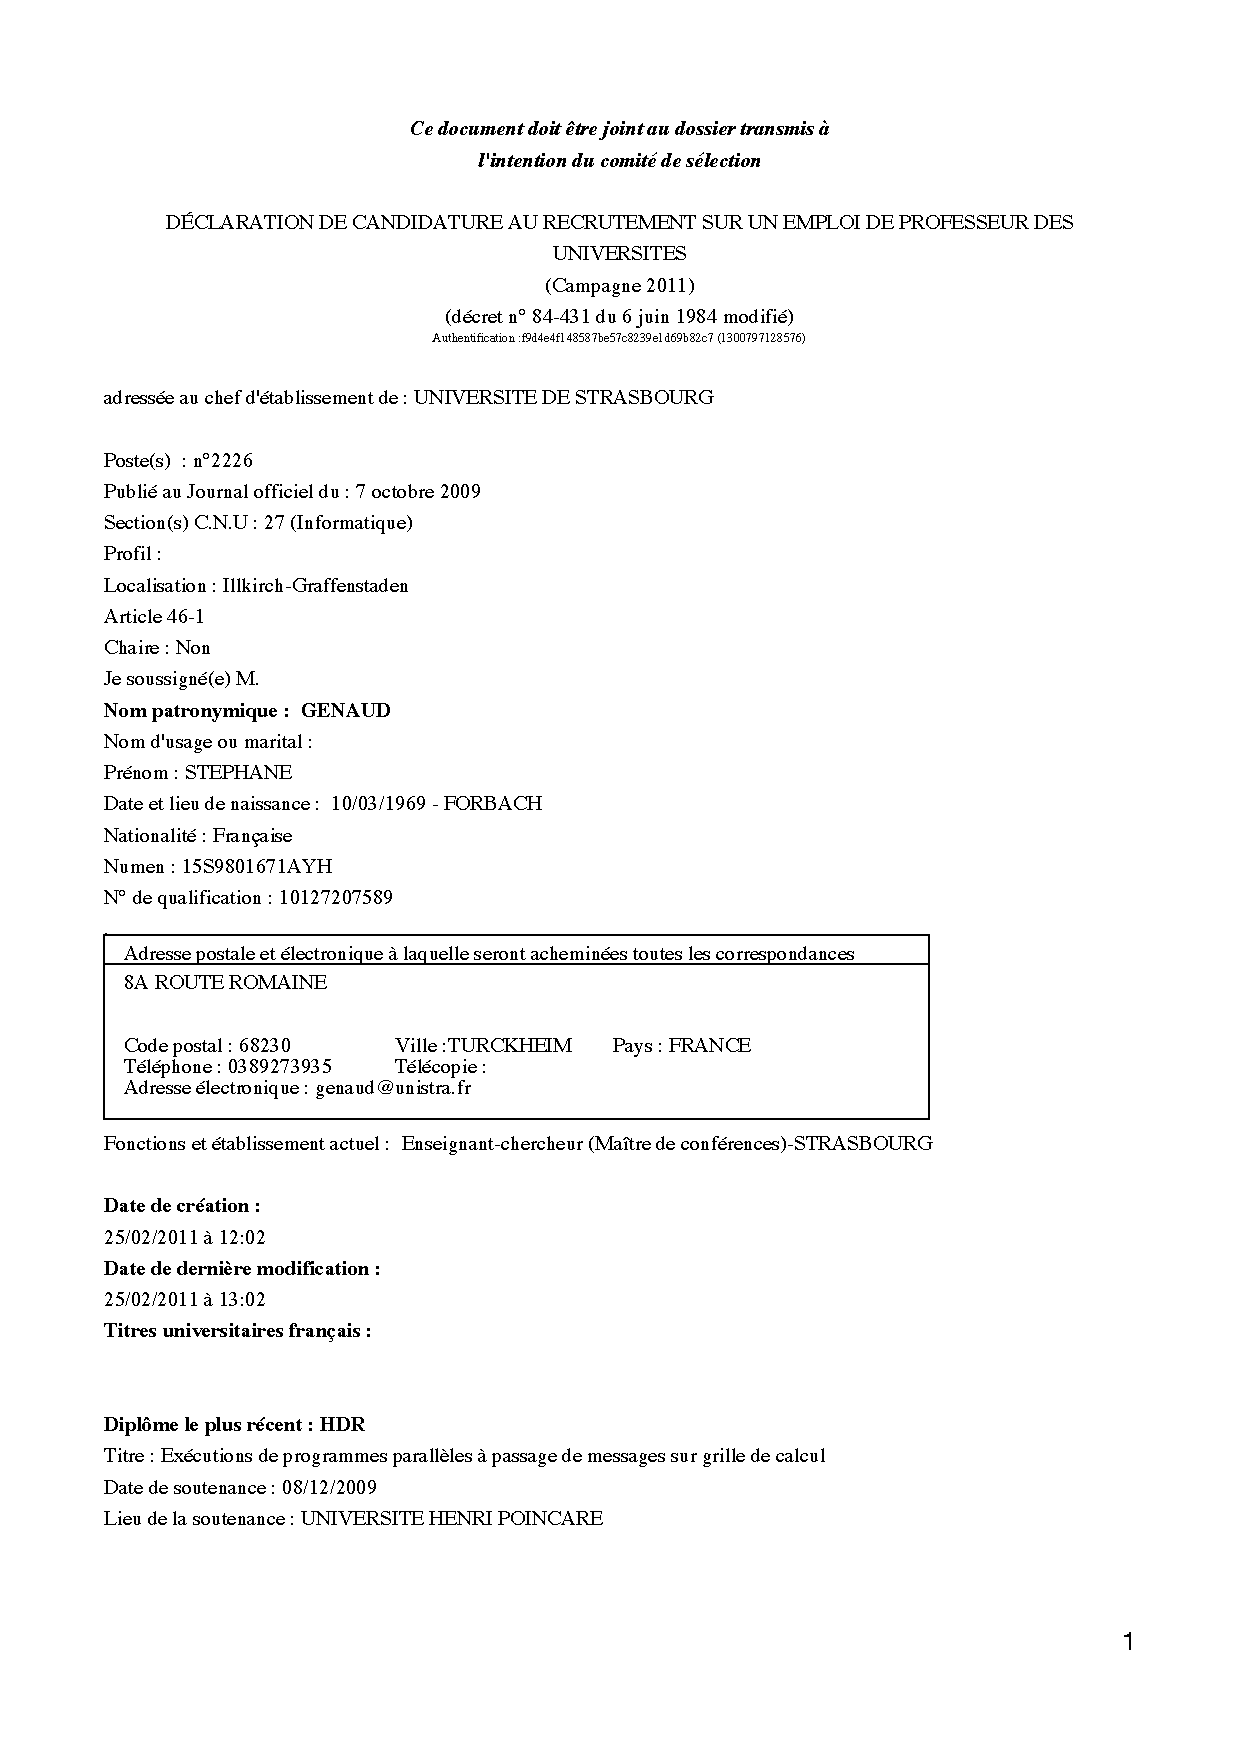
\includepdf[pages=1-2]{fiche_candidature.pdf}
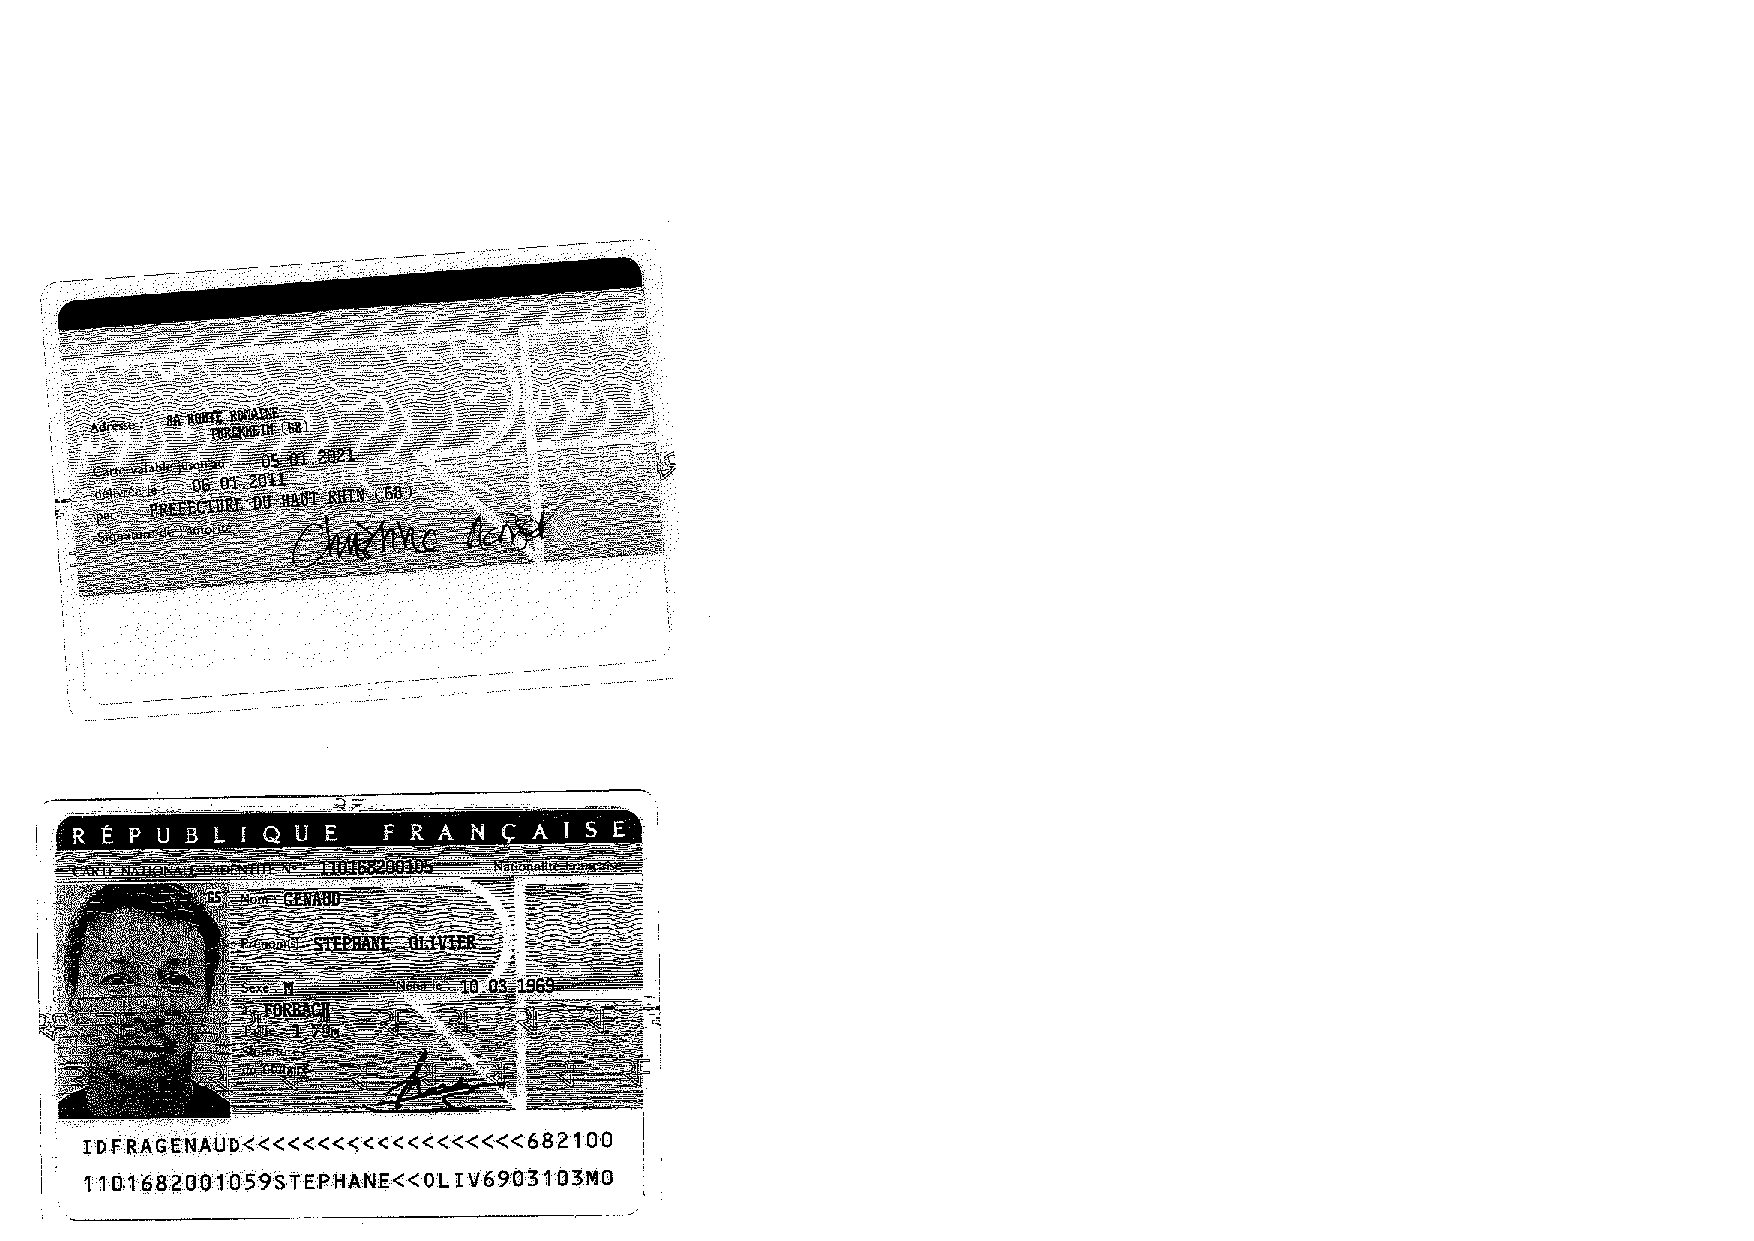
\includepdf[pages=1]{genaud_id.pdf}
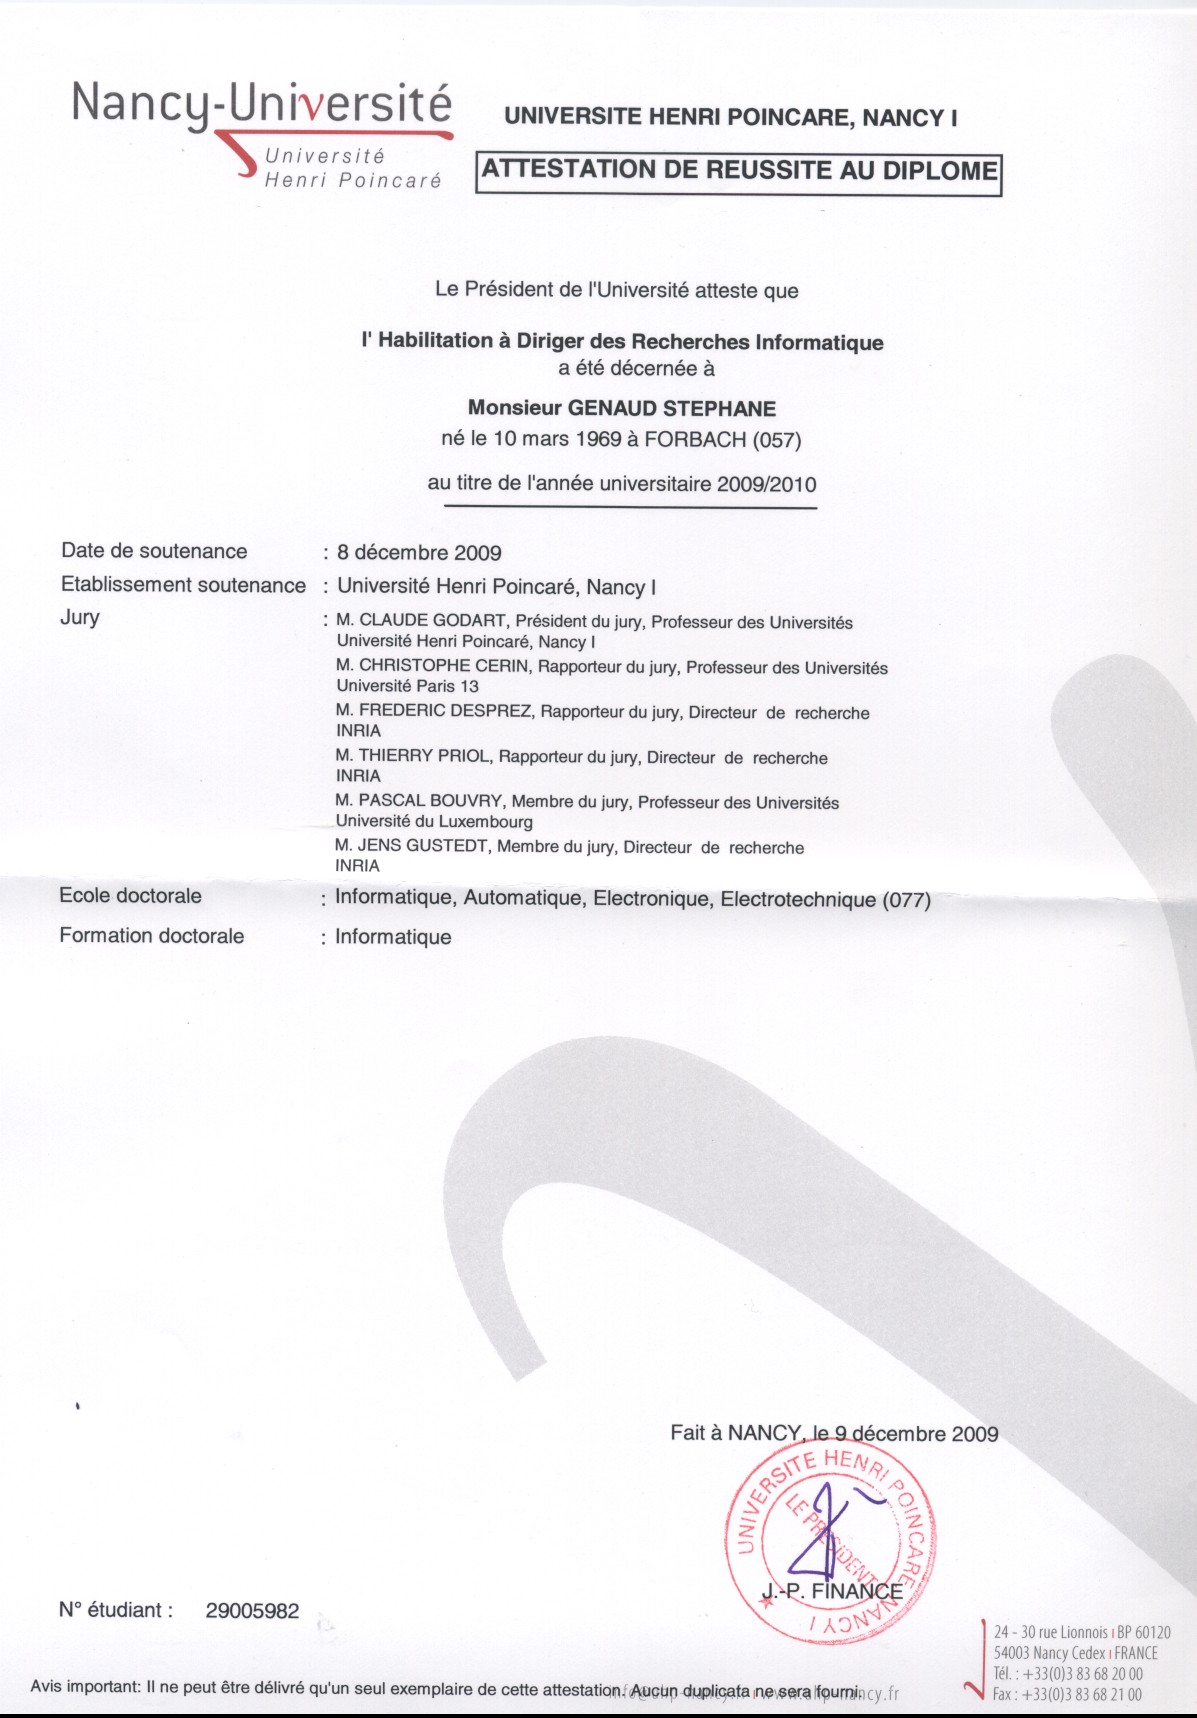
\includegraphics[height=.98\textheight]{attestation_hdr_steph.jpg}

\includepdf[pages=1]{rapport_soutenance.pdf}
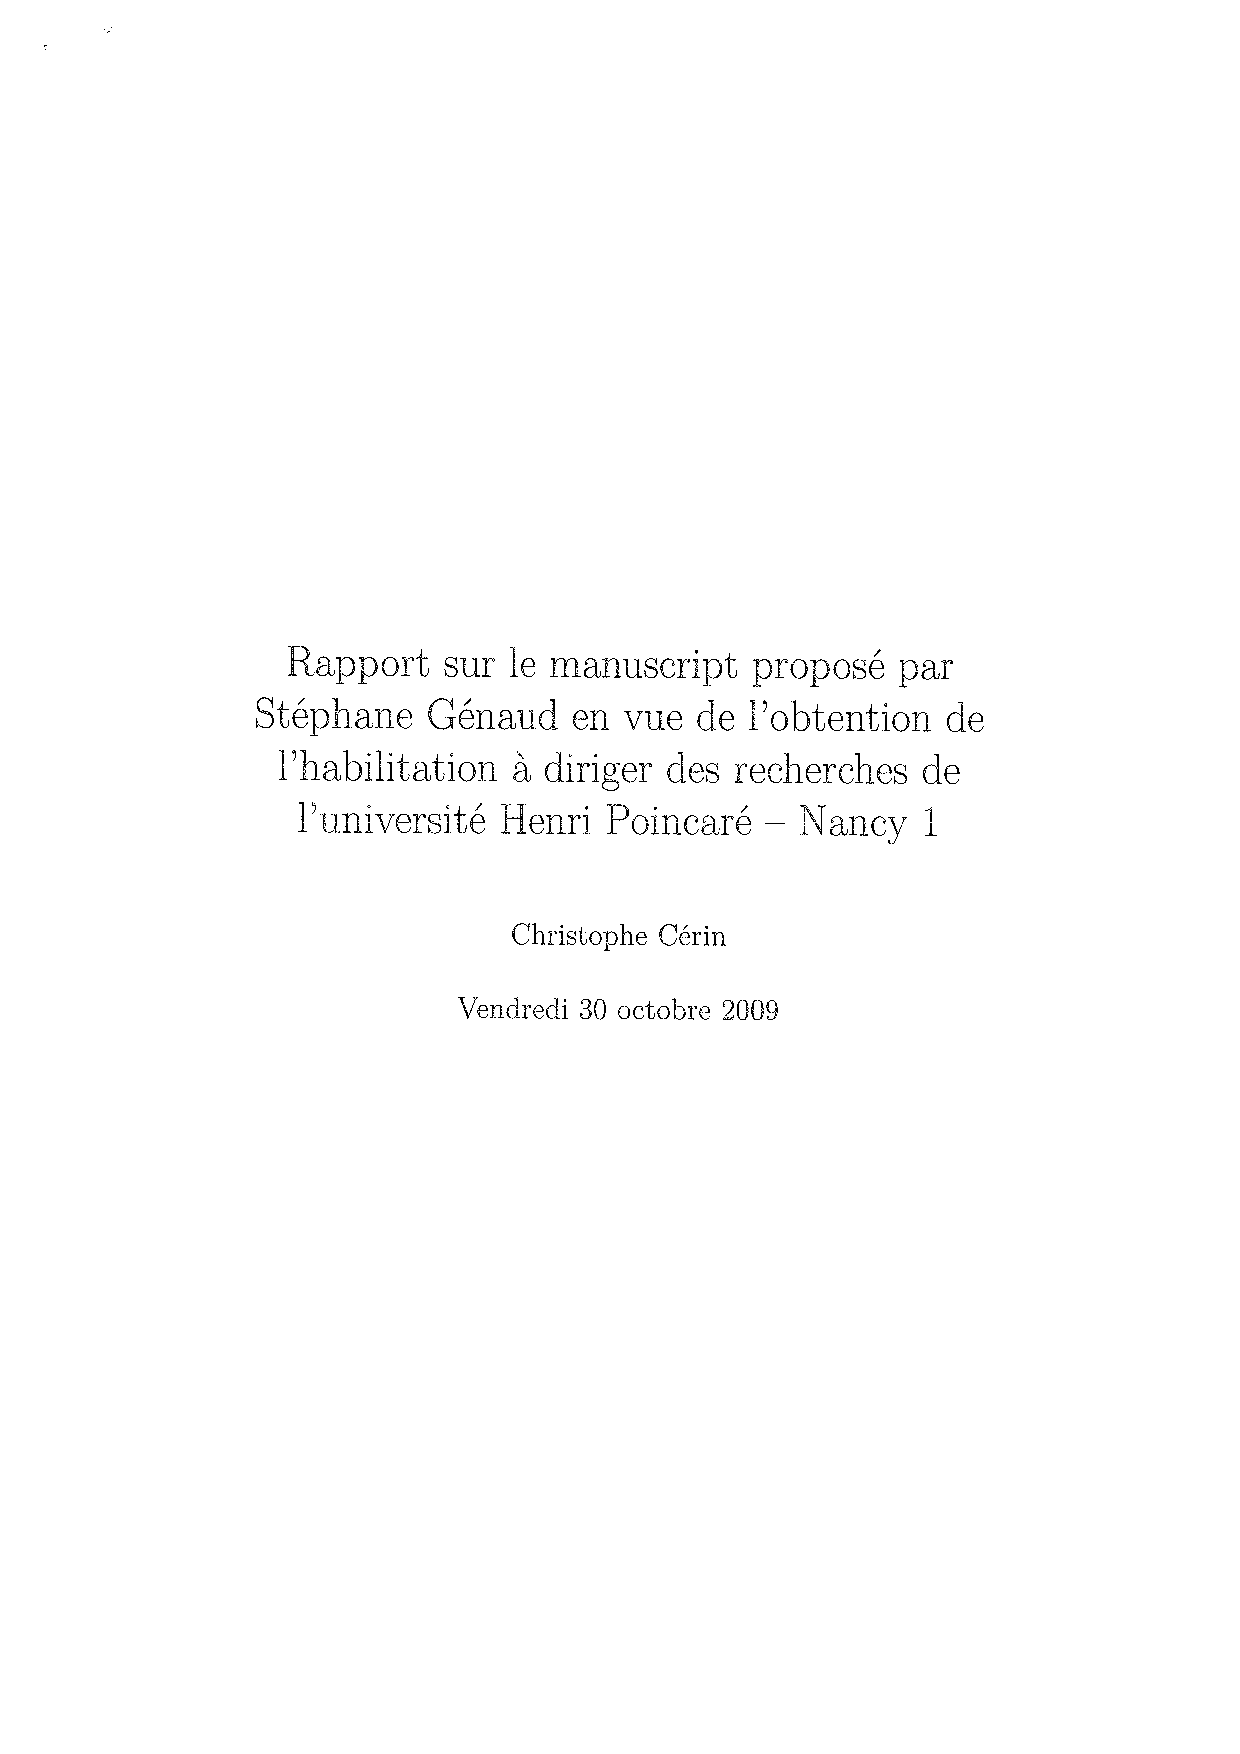
\includepdf[pages=1-5]{rapport_Cerin.pdf}
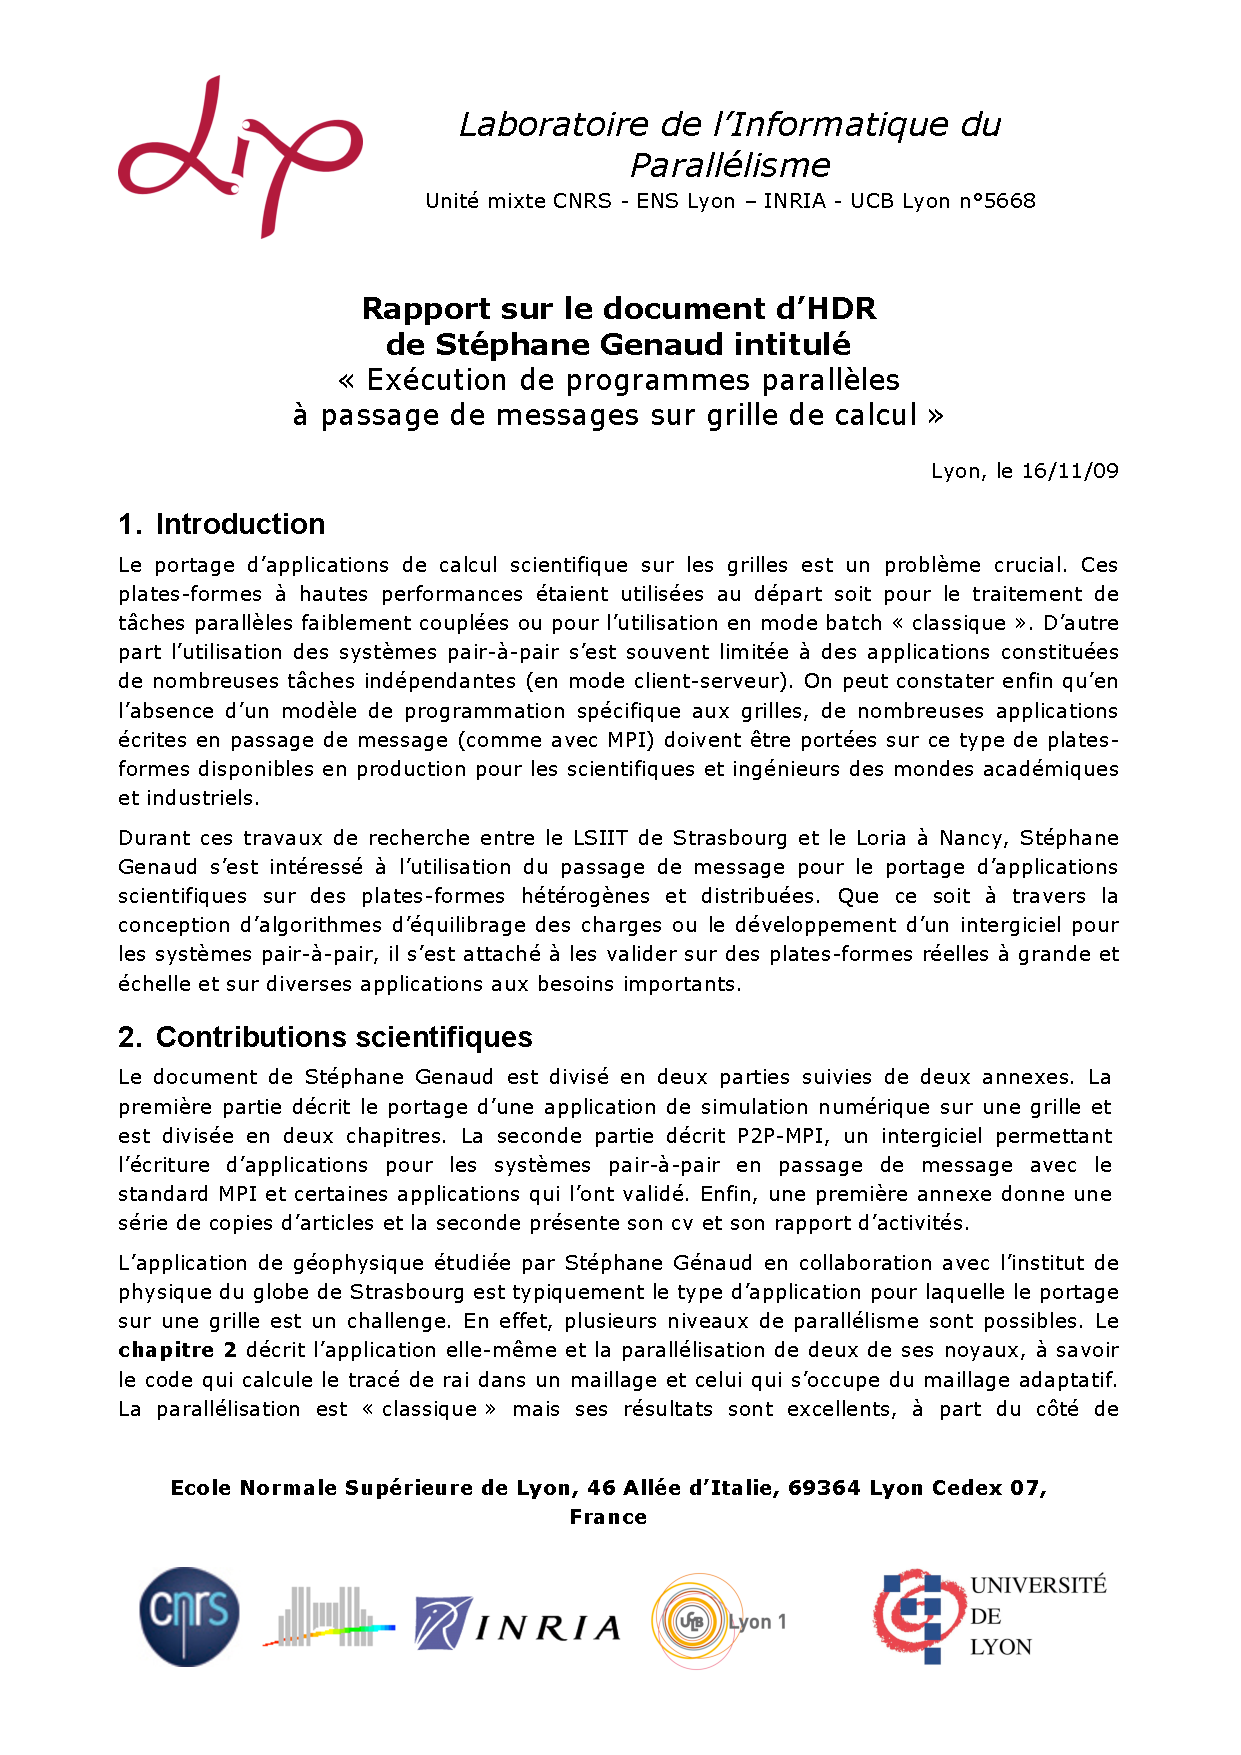
\includepdf[pages=1-2]{rapport_Desprez.pdf}
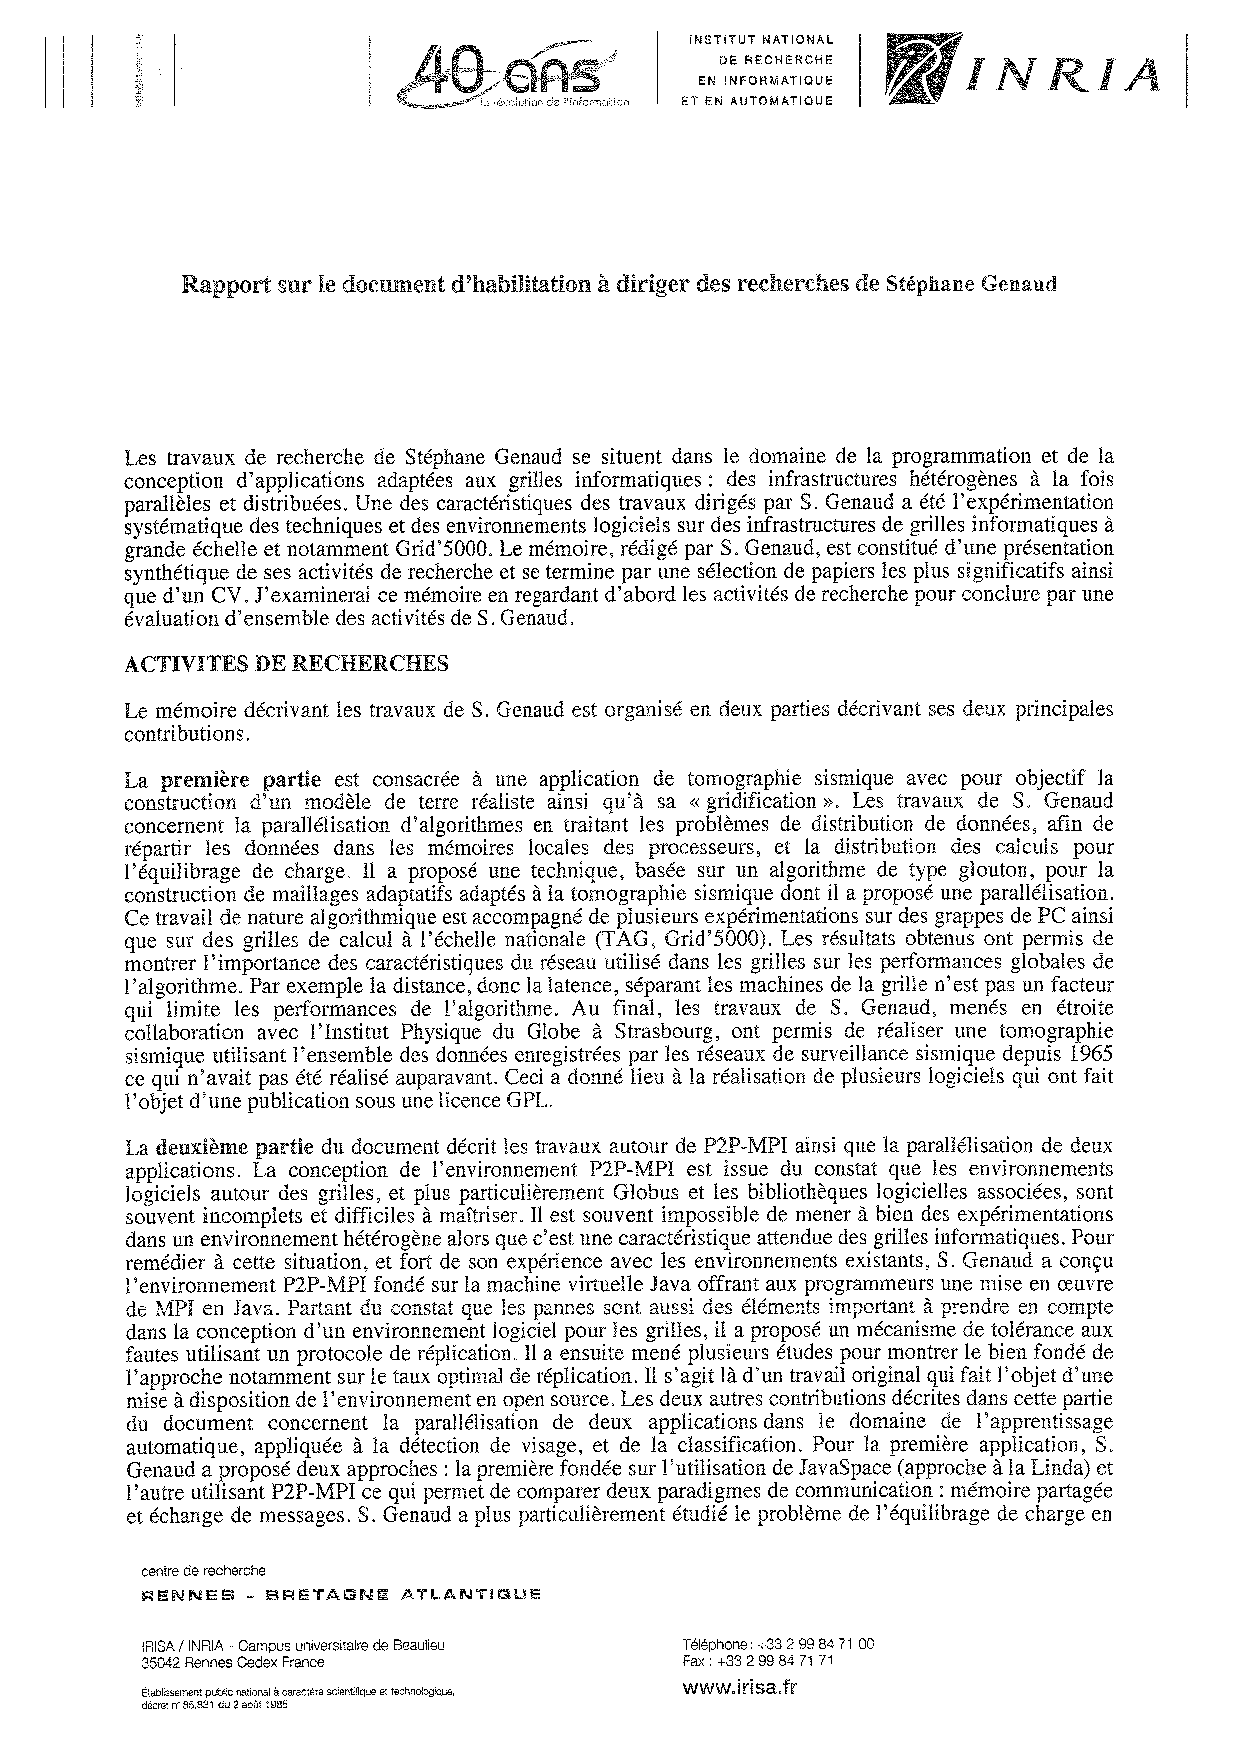
\includepdf[pages=1-2]{rapport_Priol.pdf}

\includepdf[pages=1]{reco_tellier.pdf}
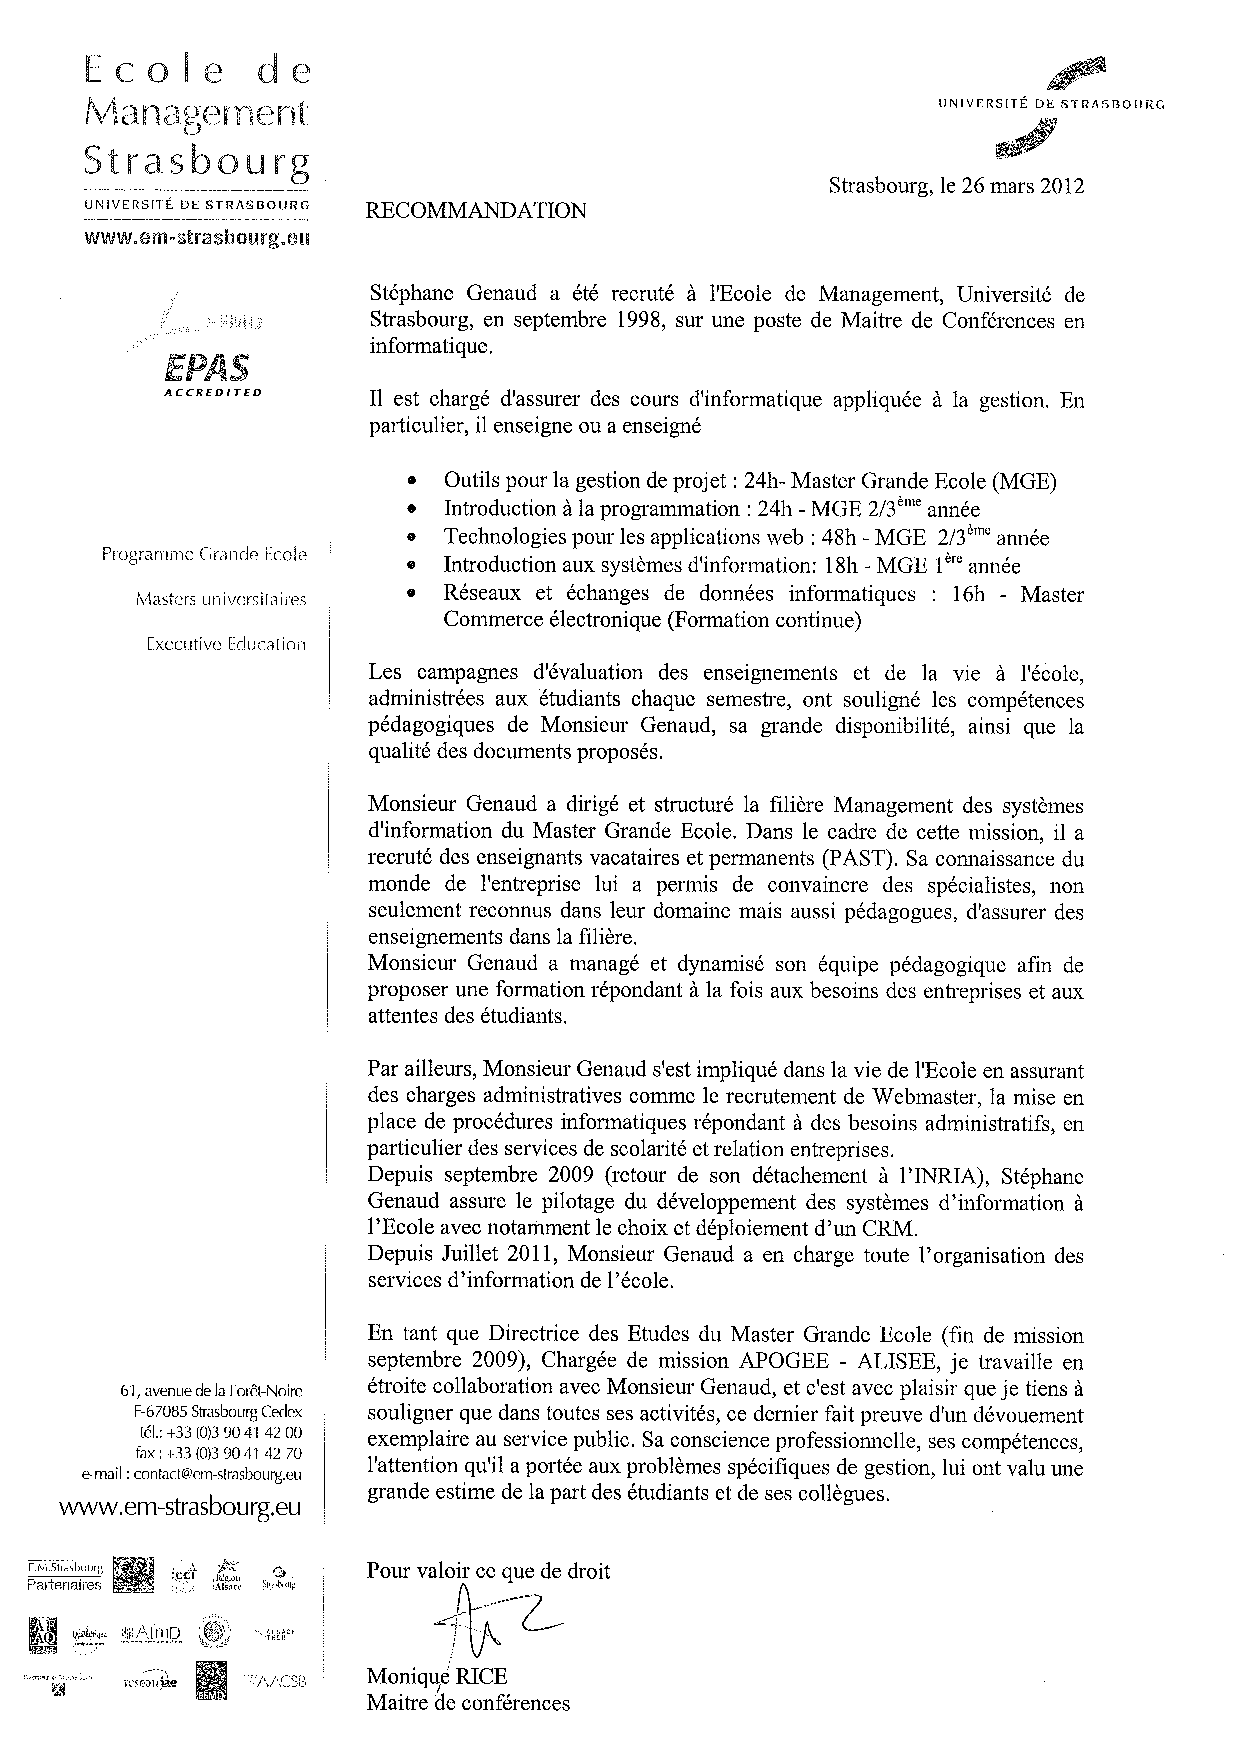
\includepdf[pages=1]{reco_rice.pdf}

\includepdf[pages=1]{reco_babak.pdf}

\includepdf[pages=1-2]{reco_jens.pdf}

%----------------------------- A R T I C L E S -------------------------------------------------------
\section{Copies d'articles}


\vspace{1cm}
Je joint ci-après six copies d'article. Ils sont classés dans un ordre chronologique inverse:

\vspace{1cm}

\begin{enumerate}
\item Article sur la simulation de programmes MPI dans le simulateur \textsc{SimGrid} (SMPI)\\
Single Node On-Line Simulation of MPI Applications with SMPI.\\
Pierre-Nicolas Clauss, Mark Stillwell, \textbf{Stéphane Genaud}, Fr\'ed\'eric Suter,\\
{\em 25th IEEE International Parallel \& Distributed Processing Symposium (IPDPS 2011)}, 
IEEE Computer Society Press, mai 2011.\\


\item Article sur la tolérance aux pannes et la détection de pannes en P2P-MPI.\\ 
Fault-Management in P2P-MPI.\\
Stéphane Genaud, Emmanuel Jeannot et Choopan Rattanapoka.\\
{\em International Journal of Parallel Programming}, Springer, 37(5):433--461, août 2009.\\


\item Article sur la parallélisation d'une méthode de clustering avec P2P-MPI.\\
Exploitation of a parallel clustering algorithm on commodity hardware with P2P-MPI.\\
Stéphane Genaud, Pierre Gançarski, Guillaume Latu, Alexandre Blansché, Choopan Rattanapoka et Damien Vouriot.\\
{\em The Journal of SuperComputing}, Springer, 43(1):21--41, jan. 2008.\\


\item Article sur la conception de P2P-MPI\\
P2P-MPI: A Peer-to-Peer Framework for Robust Execution of Message Passing Parallel Programs on Grids.
Stéphane Genaud et Choopan Rattanapoka.\\
{\em Journal of Grid Computing}, Springer, 5(1):27--42, mai 2007.\\


\item Article sur l'équilibrage de charge.\\
Load-balancing scatter operations for Grid computing.\\
Stéphane Genaud, Arnaud Giersch, et Frédéric Vivien.\\
{\em Parallel Computing}, Elsevier, 30(8):923--946, août 2004.\\


\item Article sur la parallélisation du tracé de rai de l'application de géophysique.\\
Seismic ray-tracing and Earth mesh modeling on various parallel architectures.\\
Marc Grunberg, \textbf{Stéphane Genaud} et Catherine Mongenet.\\
{\em The Journal of Supercomputing}, Kluwer, 29(1):27--44, juillet 2004.\\
\end{enumerate}

%@@@
\end{document}
\includepdf[pages=1-18]{../mypapers/Seismic-raytracing_JSC04.pdf}
%\includepdf[pages=1-8]{../mypapers/Mesh_coarsening_SBAC-PAD-04.pdf}
\includepdf[pages=1-24]{../mypapers/Load-bal-scatter_ParCo04.pdf}
\includepdf[pages=1-16]{../mypapers/P2P-MPI_joGC2007.pdf}
\includepdf[pages=1-21]{../mypapers/Parallel-clustering-P2PMPI_JSC08.pdf}
\includepdf[pages=1-28]{../mypapers/P2P-MPI-fault_management-IJPP.pdf}
\includepdf[pages=1-12]{../mypapers/IPDPS-11.pdf}






\end{document}
